\documentclass[12pt,a4paper,twoside]{report}

%--------------------------------------------------------------------------------------
% Csomagok inicializálása [Initializing packages]
%--------------------------------------------------------------------------------------
\usepackage{ifthen} % Used in macros

\usepackage{sectsty}
\usepackage[english,magyar]{babel} % Language support
\usepackage{geometry}
\usepackage{amsmath,amssymb} % Mathematical symbols
\usepackage{microtype} % Imrovements to typesetting
\usepackage{setspace} % For setting line spacing
\usepackage{cmap} % Enables more advenced text copying from the PDF document 
% \usepackage{sectsty} % Section heading styling

\usepackage[luatex,unicode]{hyperref} % For hyperlinks in the generated document
\usepackage{booktabs} % For publication quality tables for LaTeX
\usepackage{graphicx} % For figure sizing
\usepackage[hang]{caption}
\usepackage{xcolor} % For code coloring in listings
\usepackage{listings} % For source code snippets
\usepackage[amsmath,thmmarks]{ntheorem} % Theorem-like environments

\usepackage[numbers]{natbib} % Bibliography

\usepackage{fancyhdr} % For easy to use headers and footers

% thanks to http://tex.stackexchange.com/a/47579/71109
\usepackage{ifxetex}
\usepackage{ifluatex}
\newif\ifxetexorluatex % a new conditional starts as false
\ifnum 0\ifxetex 1\fi\ifluatex 1\fi>0
	\xetexorluatextrue
\fi

\ifxetexorluatex
	\usepackage{fontspec}
	% Palatino clone font (Tex Gyre Pagella) for text and math
	\usepackage{unicode-math}
	\setmainfont[Ligatures=TeX]{TeX Gyre Pagella}
	\setmathfont{TeX Gyre Pagella Math}
	\setmonofont[Scale=.85]{Menlo}
\else
	\usepackage[T1]{fontenc}
	\usepackage[utf8]{inputenc}
	%\usepackage[lighttt]{lmodern} % Advanced version of the Computer Modern font
	% Palatino clone font (Tex Gyre Pagella) for text and math
	\usepackage{tgpagella, newpxmath}
\fi

\usepackage{tikz}
\usepackage{listings}

\usepackage{mdframed}
\usepackage[print-solutions]{math-exercise}

\newmdenv[%
	backgroundcolor=yellow-base!5,%
	linecolor=blue-base,%
	linewidth=1mm,%
	topline=false,%
	rightline=false,%
	bottomline=false,%
	skipabove=0.75em,%
	skipbelow=0.75em,%
]{myframe}
\newcounter{note}
\makeatletter
\newenvironment{note}[1][\@nil]{%
	\refstepcounter{note}%
	\begin{myframe}\textbf{Megjegyzés \thenote.}%
		\def\tmp{#1}%
		\ifx\tmp\@nnil\else%
			\hspace{.5em}[\;#1\;]
		\fi\par%
		}{\end{myframe}}
\makeatother

\usepackage[abspath]{currfile}
\newcommand{\relativeinput}[1]{\input{\currfiledir#1}}
\newcommand{\relativeinclude}[1]{\input{\currfiledir#1}}
\newcommand{\relativestandalone}[1]{\includestandalone{\currfiledir#1}}

%--------------------------------------------------------------------------------------
% Elnevezések
%--------------------------------------------------------------------------------------
\newcommand{\bme}{Budapesti Műszaki és Gazdaságtudományi Egyetem}
\newcommand{\gpk}{Gépészmérnöki Kar}

\newcommand{\bmeatt}{Anyagtudomány és Technológia Tanszék}
\newcommand{\bmeara}{Áramlástan Tanszék}
\newcommand{\bmeenergia}{Energetikai Gépek és Rendszerek Tanszék}
\newcommand{\bmeepget}{Épületgépészeti és Gépészeti Eljárástechnika Tanszék}
\newcommand{\bmegtharom}{Gép- és Terméktervezés Tanszék}
\newcommand{\bmemanuf}{Gyártástudomány és -technológia Tanszék}
\newcommand{\bmehds}{Hidrodinamikai Rendszerek Tanszék}
\newcommand{\bmemogi}{Mechatronika, Optika és Gépészeti Informatika Tanszék}
\newcommand{\bmemm}{Műszaki Mechanika Tanszék}
\newcommand{\bmept}{Polimertechnika Tanszék}

\newcommand{\keszitette}{Készítette}
\newcommand{\konzulens}{Konzulens}
\newcommand{\temavezeto}{Témavezető}

\newcommand{\selectbsc}{
  \newcommand{\gpkmunkatipus}{Szakdolgozat}       % Dokumentum típusa [Document type]
  \newcommand{\gpkmunkatipusHU}{Szakdolgozat}     % Dokumentum típusa HU
  \newcommand{\gpkmunkatipusok}{Szakdolgozatok}   % többesszámban
  \newcommand{\gpkmunkatipustHU}{Szakdolgozatot}  % tárgyraggal
}
\newcommand{\selectmsc}{
  \newcommand{\gpkmunkatipus}{Diplomaterv}        % Dokumentum típusa [Document type]
  \newcommand{\gpkmunkatipusHU}{Diplomaterv}      % Dokumentum típusa HU
  \newcommand{\gpkmunkatipusok}{Diplomatervek}    % többesszámban
  \newcommand{\gpkmunkatipustHU}{Diplomatervet}   % tárgyraggal
}

\newcommand{\tdk}{TDK dolgozat}
\newcommand{\bsconlab}{BSc Önálló laboratórium}
\newcommand{\msconlabi}{MSc Önálló laboratórium 1.}
\newcommand{\msconlabii}{MSc Önálló laboratórium 2.}

\newcommand{\szerzoijog}{Szerzői jog}

\newcommand{\pelda}{Példa}
\newcommand{\definicio}{Definíció}
\newcommand{\tetel}{Tétel}

\newcommand{\jelolesek}{Jelölések jegyzéke}
\newcommand{\eloszo}{Előszó}
\newcommand{\bevezetes}{Bevezetés}
\newcommand{\koszonetnyilvanitas}{Köszönetnyilvánítás}
\newcommand{\osszefoglalas}{Összefoglalás}
\newcommand{\summary}{Summary}
\newcommand{\fuggelek}{Függelék}
\newcommand{\melleklet}{Mellékletek}

% Opcionálisan átnevezhető címek
\addto\captionsmagyar{%
\renewcommand{\listfigurename}{Illusztrációk jegyzéke}
%\renewcommand{\listtablename}{Saját táblázatjegyzék cím}
%\renewcommand{\bibname}{Saját irodalomjegyzék név}
}

\newcommand{\authorName}{\authorFamilyName{} \authorGivenName}
\newcommand{\consulentA}{\consulentATitle\consulentAFamilyName{} \consulentAGivenName}
\newcommand{\consulentB}{\consulentBTitle\consulentBFamilyName{} \consulentBGivenName}
\newcommand{\consulentC}{\consulentCTitle\consulentCFamilyName{} \consulentCGivenName}
\newcommand{\supervisor}{\supervisorTitle\supervisorFamilyName{}
\supervisorGivenName}

\newcommand{\selectthesislanguage}{\selecthungarian}
\newcommand{\selectforeignlanguage}{\selectenglish}

\bibliographystyle{huplain}

\def\lstlistingname{lista}

\newcommand{\appendixletter}{6} % a fofejezet-szamlalo az angol ABC 6. betuje (F) lesz
\newcommand{\annexletter}{13} % M betű

%-------------------------------------------------------------------------------
% Page layout setup
%-------------------------------------------------------------------------------
% we need to redefine the pagestyle plain
% another possibility is to use the body of this command without \fancypagestyle
% and use \pagestyle{fancy} but in that case the special pages
% (like the ToC, the References, and the Chapter pages)remain in plane style

\pagestyle{plain}
\geometry{inner=30mm, outer=20mm, top=20mm, bottom=30mm}


%-------------------------------------------------------------------------------
% Text and paragraph styling
%-------------------------------------------------------------------------------

\sectionfont{\Large\upshape\bfseries}  % Section title font
\subsectionfont{\Large\itshape\mdseries}
\subsubsectionfont{\large\itshape\mdseries}
\setcounter{secnumdepth}{3}             % Section numbering depth

\sloppy                                 % Prevent text from spilling over the margin
\widowpenalty=10000 \clubpenalty=10000  % Prevent widow and oprhan rows
\def\hyph{-\penalty0\hskip0pt\relax}    % Enable hyphenation

\onehalfspacing                         % 1.5x Line spacing

% Text setup for Hungarian text
\newcommand{\selecthungarian}{
	\selectlanguage{magyar}
	\setlength{\parindent}{2em}			% Paragraph indentation
	\setlength{\parskip}{5pt}			% Paragraph spacing
	\frenchspacing
}

% Text setup for English text
\newcommand{\selectenglish}{
	\selectlanguage{english}
	\setlength{\parindent}{0em}
	\setlength{\parskip}{8pt}
	\nonfrenchspacing
}

%-------------------------------------------------------------------------------
% Setup hyperref package
%-------------------------------------------------------------------------------
\hypersetup{
	% bookmarks=true,            % show bookmarks bar?
	unicode=true,                % non-Latin characters in Acrobat's bookmarks
	pdfnewwindow=true,           % links in new window
	colorlinks=true,             % false: boxed links; true: colored links
	linkcolor=black,             % color of internal links
	citecolor=black,             % color of links to bibliography
	filecolor=black,             % color of file links
	urlcolor=black               % color of external links
}

%-------------------------------------------------------------------------------
% Apply variables
%-------------------------------------------------------------------------------
% This command is called in the main tex file and uses variables set there.
\newcommand{\applyvariables}{
	\author{\authorName}
	\title{\thesisTitle}

	\hypersetup{
		pdftitle={\thesisTitle},     % title
		pdfauthor={\authorName},     % author
		pdfsubject={\gpkmunkatipus}, % subject of the document
		pdfkeywords={\keywords},     % list of keywords (separate then by comma)
		pdfproducer={\authorName},   % producer of the document (organization)
		pdfcreator={LaTeX}           % creator of the document (application)
	}
}

%-------------------------------------------------------------------------------
% Set up listings
%-------------------------------------------------------------------------------
\definecolor{lightgray}{rgb}{0.95,0.95,0.95}
\lstset{
basicstyle=\scriptsize\ttfamily, % print whole listing small
keywordstyle=\color{black}\bfseries, % bold black keywords
identifierstyle=, % nothing happens
% default behavior: comments in italic, to change use
% commentstyle=\color{green}, % for e.g. green comments
% stringstyle=\scriptsize,
stringstyle=\normalsize,
showstringspaces=false, % no special string spaces
aboveskip=10pt,
belowskip=10pt,
backgroundcolor=\color{lightgray},
columns=flexible,
keepspaces=true,
escapeinside={(*@}{@*)},
captionpos=b,
breaklines=true,
frame=single,
float=!ht,
tabsize=2,
literate=*
	{á}{{\'a}}1	{é}{{\'e}}1	{í}{{\'i}}1	{ó}{{\'o}}1	{ö}{{\"o}}1	{ő}{{\H{o}}}1	{ú}{{\'u}}1	{ü}{{\"u}}1	{ű}{{\H{u}}}1
{Á}{{\'A}}1	{É}{{\'E}}1	{Í}{{\'I}}1	{Ó}{{\'O}}1	{Ö}{{\"O}}1	{Ő}{{\H{O}}}1	{Ú}{{\'U}}1	{Ü}{{\"U}}1	{Ű}{{\H{U}}}1
}


%-------------------------------------------------------------------------------
% Set up theorem-like environments
%-------------------------------------------------------------------------------
% Using ntheorem package -- see http://www.math.washington.edu/tex-archive/macros/latex/contrib/ntheorem/ntheorem.pdf

\theoremstyle{plain}
\theoremseparator{.}
\newtheorem{example}{\pelda}

\theoremseparator{.}
%\theoremprework{\bigskip\hrule\medskip}
%\theorempostwork{\hrule\bigskip}
\theorembodyfont{\upshape}
\theoremsymbol{{\large \ensuremath{\centerdot}}}
\newtheorem{definition}{\definicio}

\theoremseparator{.}
%\theoremprework{\bigskip\hrule\medskip}
%\theorempostwork{\hrule\bigskip}
\newtheorem{theorem}{\tetel}


%-------------------------------------------------------------------------------
% Some new commands and declarations
%-------------------------------------------------------------------------------
\newcommand{\code}[1]{{\upshape\ttfamily\scriptsize\indent #1}}
\newcommand{\doi}[1]{DOI: \href{http://dx.doi.org/\detokenize{#1}}{\raggedright{\texttt{\detokenize{#1}}}}} % A hivatkozások közt így könnyebb DOI-t megadni.

\DeclareMathOperator*{\argmax}{arg\,max}
%\DeclareMathOperator*[1]{\floor}{arg\,max}
\DeclareMathOperator{\sign}{sgn}
\DeclareMathOperator{\rot}{rot}


%-------------------------------------------------------------------------------
% Setup captions
%-------------------------------------------------------------------------------
\captionsetup[figure]{
	width=.75\textwidth,
	aboveskip=10pt
}

\renewcommand{\captionlabelfont}{\it}
\renewcommand{\captionfont}{\footnotesize\it}

%-------------------------------------------------------------------------------
% Hyphenation exceptions
%-------------------------------------------------------------------------------
\hyphenation{Shakes-peare Mar-seilles ár-víz-tű-rő tü-kör-fú-ró-gép}


%-------------------------------------------------------------------------------
% Command to exclude tables and images in the annex from the List of Figures/Tables
%-------------------------------------------------------------------------------
\newcommand{\excludeFromLocAndLot}{
	% Redefine \addcontentsline to be silent when printing loc or toc entries
	\let\svaddcontentsline\addcontentsline
	\renewcommand\addcontentsline[3]{
		\ifthenelse{\equal{##1}{lof}}{}{
			\ifthenelse{\equal{##1}{lot}}{}{
				\svaddcontentsline{##1}{##2}{##3}
			}
		}
	}
}

% Own commands
\newcommand{\inlinecode}[1]{\texttt{`#1`}}


\selectbsc    % Szakdolgozat [Bachelor's]

\def\authorFamilyName{Sándor}
\def\authorGivenName{Tibor}
\def\neptun{C7XUDE}

\def\consulentATitle{dr.~}
\def\consulentAFamilyName{Koós}
\def\consulentAGivenName{Krisztiánné}
\def\consulentARank{docens}

\def\consulentBTitle{}
\def\consulentBFamilyName{}
\def\consulentBGivenName{}
\def\consulentBRank{}

\def\consulentCTitle{}
\def\consulentCFamilyName{}
\def\consulentCGivenName{}
\def\consulentCRank{}

% Témavezető
\def\supervisorTitle{dr.~}
\def\supervisorFamilyName{Budai}
\def\supervisorGivenName{Csaba}
\def\supervisorRank{adjunktus}

% Dolgozat címe [Thesis title]
\def\thesisTitle{Új Tanuláselméleti Eredményekkel Támogatott Oktatási Anyagok Fejlesztése és Alkalmazása}

\def\keywords{mechatronika, matematika}

\def\department{\bmemogi}

\def\endOfRestrictedAccess{... év ... hónap ... nap}

\applyvariables


%--------------------------------------------------------------------------------------
% Dokumentum törzse [Document body]
%--------------------------------------------------------------------------------------

\begin{document}

\pagenumbering{gobble}
\selectthesislanguage

% Címoldal [Titlepage]
\hypersetup{pageanchor=false}

%--------------------------------------------------------------------------------------
% Szennycímoldal [Cover title page]
%--------------------------------------------------------------------------------------

\clearpage
\begin{center}
\MakeUppercase{\authorName}\\[0.1cm]
\MakeUppercase{\gpkmunkatipus}\\[0.1cm]
\end{center}
\thispagestyle{empty}

%--------------------------------------------------------------------------------------
% Sorozatcímoldal [Series title page]
%--------------------------------------------------------------------------------------
\clearpage
\begin{center}


\includegraphics[width=60mm,keepaspectratio]{figures/bme_logo.pdf}\\
\vspace{0.3cm}
\MakeUppercase{\textbf{\bme}}\\[0.1cm]
\MakeUppercase{\textmd{\gpk}}\\[0.1cm]
\MakeUppercase{\textmd{\department}}\\[0.8cm]


\includegraphics[height=40mm,keepaspectratio]{figures/tanszek_logo}\\[0.5cm]
\MakeUppercase{\gpkmunkatipusok}

\end{center}
\thispagestyle{empty}

%--------------------------------------------------------------------------------------
% Címoldal [Title page]
%--------------------------------------------------------------------------------------
\begin{titlepage}
\begin{center}

\includegraphics[width=60mm,keepaspectratio]{figures/bme_logo.pdf}\\
\vspace{0.3cm}
\MakeUppercase{\textbf{\bme}}\\[0.1cm]
\MakeUppercase{\textmd{\gpk}}\\[0.1cm]
\MakeUppercase{\textmd{\department}}

\vspace{4.0cm}
{\huge \textsc{\authorName}}\\[0.8cm]
{\huge \MakeUppercase{\gpkmunkatipus}}\\[0.8cm]
{\Large \thesisTitle}

\vspace{3.0cm}

{
	\renewcommand{\arraystretch}{0.85}
	\begin{tabular}{ll}
	 \makebox[7cm][l]{\konzulens:} & \makebox[7cm][l]{\temavezeto:} \\
	 \noalign{\smallskip}
	 \makebox[7cm][l]{\hspace{1cm}\emph{\consulentA}} & \makebox[7cm][l]{\hspace{1cm}\emph{\supervisor}} \\
	 \makebox[7cm][l]{\hspace{1cm}\consulentARank} & \makebox[7cm][l]{\hspace{1cm}\supervisorRank} \\
	 \\
	 \makebox[7cm][l]{\hspace{1cm}\emph{\consulentB}} & \\
	 \makebox[7cm][l]{\hspace{1cm}\consulentBRank} & \\
	 \\
	 \makebox[7cm][l]{\hspace{1cm}\emph{\consulentC}} & \\
	 \makebox[7cm][l]{\hspace{1cm}\consulentCRank} & \\
	 
	\end{tabular}
}

\vfill
{\Large Budapest, \the\year.}
\end{center}
\end{titlepage}
\hypersetup{pageanchor=false}
\thispagestyle{empty}
  % Szakdolgozat/Diplomaterv címlap [Thesis]


% Copytightoldal [Copyright page]
%TODO Válaszd ki a megfelelőt! [Choose one]
\selectlanguage{magyar}
\pagenumbering{gobble}
\selecthungarian
%--------------------------------------------------------------------------------------
% Copyrightoldal
%--------------------------------------------------------------------------------------
\begin{flushleft}
\szerzoijog{} {\textcopyright} \authorName, \the\year.
\end{flushleft}

\vfill
\clearpage
\thispagestyle{empty} % an empty page

\selectthesislanguage
               % Nyílt kezelésű [Open access]
%\selectlanguage{magyar}
\pagenumbering{gobble}
\selecthungarian
%-------------------------------------------------------------------------------
% Copyrightoldal
%-------------------------------------------------------------------------------
\begin{flushleft}
  Szerzői jog {\textcopyright} \authorName, \the\year.
\end{flushleft}

\vspace{0.5cm}

\begin{center}
  \textbf{ZÁRADÉK}\\
\end{center}

\vspace{0.5cm}
\noindent
Ez a \MakeLowercase{\gpkmunkatipusHU} elzártan kezelendő és őrzendő, a
hozzáférése a vonatkozó szabályok szerint korlátozott, a dolgozat tartalmát
csak az arra feljogosított személyek ismerhetik.

A korlátozott hozzáférés időtartamának lejártáig az arra feljogosítottakon kívül
csak a korlátozást kérelmező személy vagy gazdálkodó szervezet írásos
engedélyéjével rendelkező személy nyerhet betekintést a dolgozat tartalmába.

\vspace{0.3cm}

A hozzáférés korlátozása és a zárt kezelés \endOfRestrictedAccess ján ér véget.

\vfill
\clearpage
\thispagestyle{empty}

\selectthesislanguage
   % Elzárt kezelésű [Restricted access]


% Feladatkiírás [Project page]
%TODO A nyomtatott verzóban ne szerepeljen! [Remove before printing]
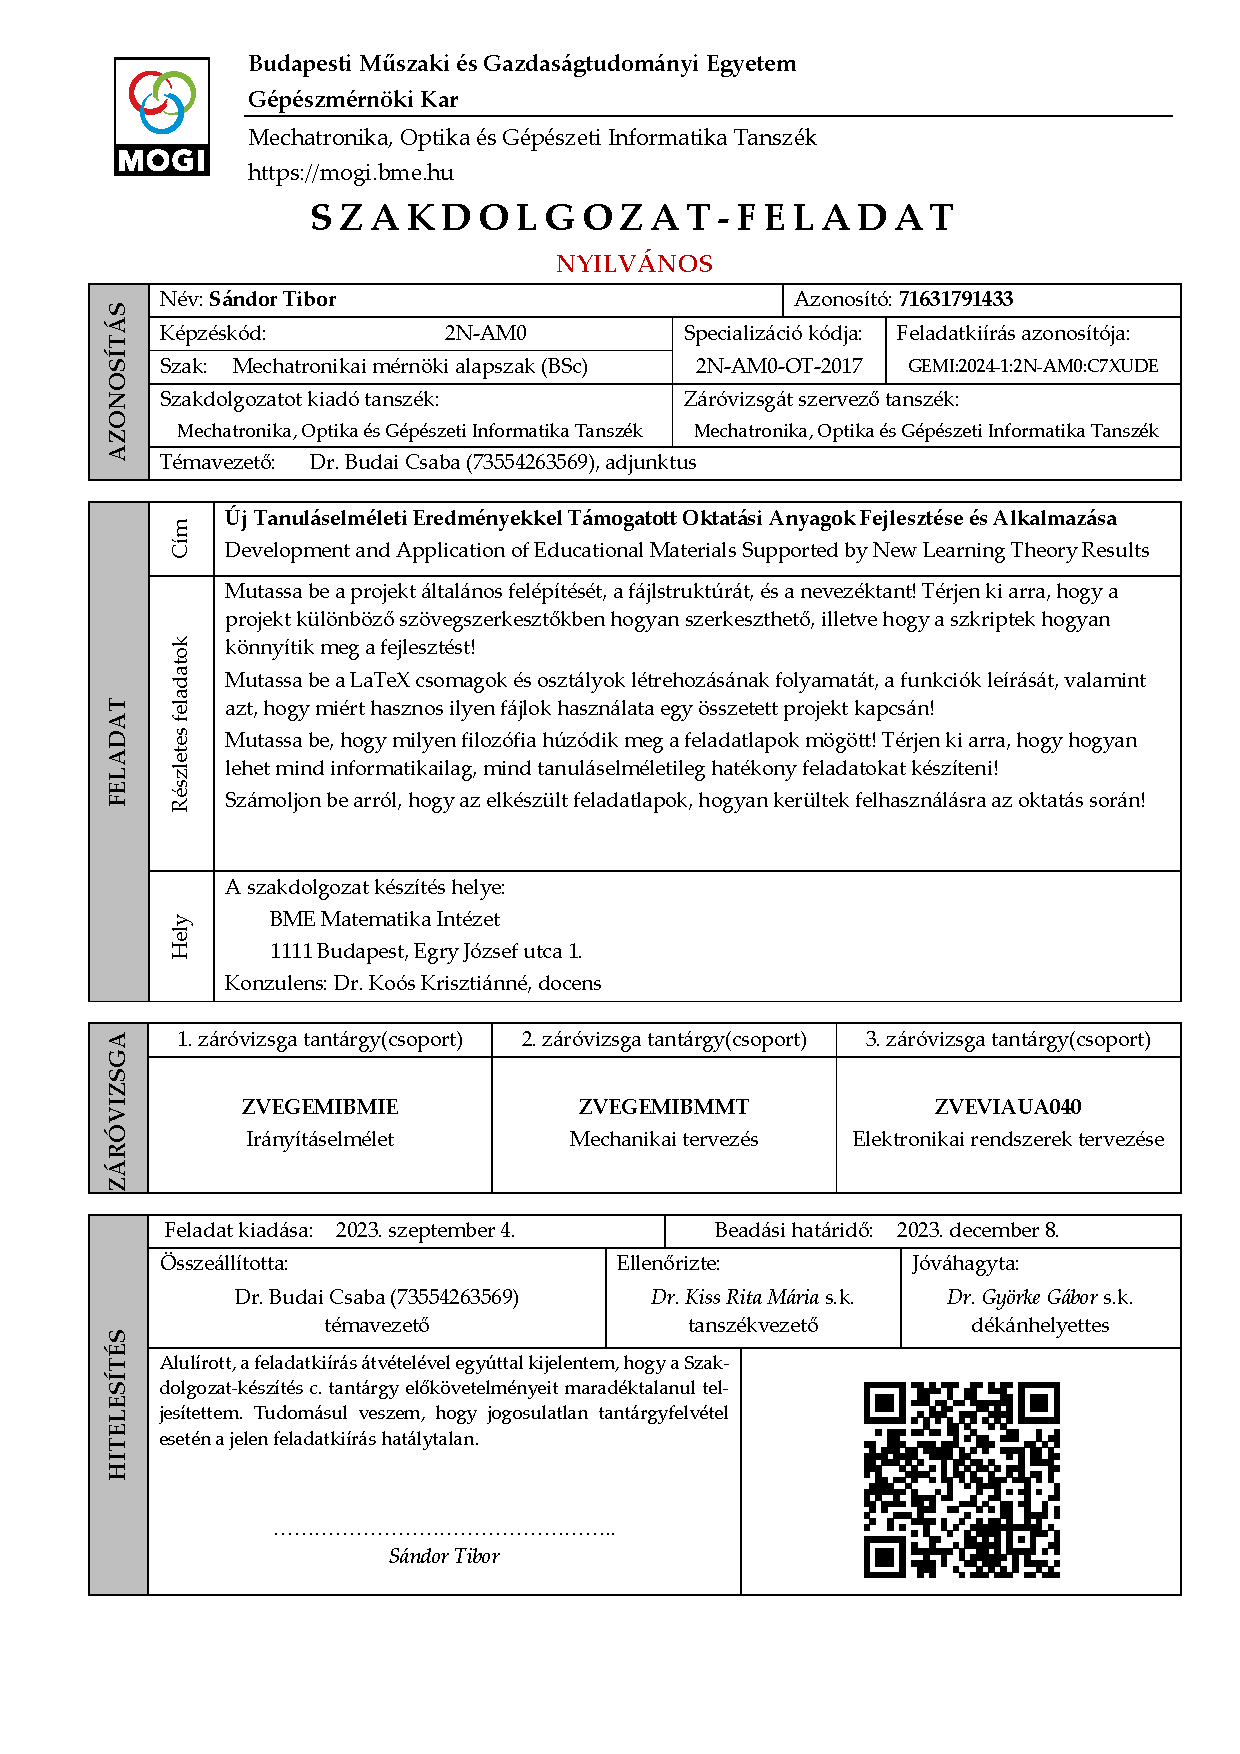
\includepdf[pages=-]{./figures/MOGI_SZD_C7XUDE_23o.pdf}



% Nyilatkozatok [Declarations]
\selectlanguage{magyar}
\selecthungarian
\pagenumbering{roman}
\setcounter{page}{6}
\cleardoublepage % duplexnél páratlan oldalon legyen
%--------------------------------------------------------------------------------------
% Nyilatkozatok
%--------------------------------------------------------------------------------------
\begin{center}
\section*{NYILATKOZATOK}
\end{center}

\vspace{0.5cm}

\begin{center}
\emph{Beadhatósági nyilatkozat}
\end{center}
A jelen \MakeLowercase{\gpkmunkatipusHU} az üzem/intézmény által elvárt szakmai színvonalnak mind tartalmilag, mind formailag megfelel, beadható.

\begin{flushleft}
Kelt,
\end{flushleft}

\begin{flushright}
 \makebox[7cm][l]{Az üzem részéről:}\\
 \vspace{0.5cm}
 \makebox[7cm]{\rule{6cm}{.4pt}}\\
 \makebox[7cm]{\emph{üzemi konzulens}}
\end{flushright}
\vspace{0.6cm}

%--------------------------------------------------------------------------------------

\begin{center}
\emph{Elfogadási nyilatkozat}
\end{center}
Ezen \MakeLowercase{\gpkmunkatipusHU} a Budapesti Műszaki és Gazdaságtudományi Egyetem Gépészmérnöki Kara által a Diplomatervezési és Szakdolgozat feladatokra előírt valamennyi tartalmi és formai követelménynek, továbbá a feladatkiírásban előírtaknak maradéktalanul eleget tesz. E \MakeLowercase{\gpkmunkatipustHU} a nyilvános bírálatra és nyilvános előadásra alkalmasnak tartom.

\begin{flushleft}
A beadás időpontja:
\end{flushleft}

\begin{flushright}
 \makebox[7cm]{\rule{6cm}{.4pt}}\\
 \makebox[7cm]{\emph{témavezető}}
\end{flushright}
\vspace{0.6cm}

%--------------------------------------------------------------------------------------

\begin{center}
\emph{Nyilatkozat az önálló munkáról}
\end{center}
Alulírott,  \emph{\authorFamilyName{} \authorGivenName} (\neptun), a Budapesti Műszaki és Gazdaságtudományi Egyetem hallgatója, büntetőjogi és fegyelmi felelősségem tudatában kijelentem és sajátkezű aláírásommal igazolom, hogy ezt a \MakeLowercase{\gpkmunkatipustHU} meg nem engedett segítség nélkül, saját magam készítettem, és dolgozatomban csak a megadott forrásokat használtam fel. Minden olyan részt, melyet szó szerint vagy azonos értelemben, de átfogalmazva más forrásból átvettem, egyértelműen, a hatályos előírásoknak megfelelően, a forrás megadásával megjelöltem.

\begin{flushleft}
Budapest, \today
\end{flushleft}

\begin{flushright}
 \makebox[7cm]{\rule{6cm}{.4pt}}\\
 \makebox[7cm]{\emph{hallgató}}
\end{flushright}


\vfill
\clearpage

\selectthesislanguage

\newcounter{romanPage}
\setcounter{romanPage}{\value{page}}
\stepcounter{romanPage}


\selectthesislanguage
\setcounter{tocdepth}{3}
\tableofcontents\vfill

\listoffigures\addcontentsline{toc}{chapter}{\listfigurename}
\listoftables\addcontentsline{toc}{chapter}{\listtablename}
\renewcommand\lstlistingname{kódrészlet}
\renewcommand\lstlistlistingname{Kódrészletek jegyzéke}
\lstlistoflistings\addcontentsline{toc}{chapter}{\lstlistlistingname}

%-------------------------------------------------------------------------------
\chapter*{\eloszo}\addcontentsline{toc}{chapter}{\eloszo}
%-------------------------------------------------------------------------------

A COVID-19 világjárvány oktatásra gyakorolt tartós hatása várhatóan még hosszú
évekig érezhető lesz. Azok a hallgatók, akik 2022-ben kezdték meg egyetemi
tanulmányaikat azzal a kihívással szembesültek, hogy középiskolai tanulmányaikat
a járvány tetőpontján fejezték be, amely egy döntő fontosságú időszak
tanulmányaik szempontjából. A korábbi évekhez képest a Matematika G1
tantárgy vizsgáinak átmeneti aránya jelentősen csökkent, annak ellenére,
hogy rendelkezésre álltak különböző segédeszközök, például interaktív online
felületek, oktatófilmek, átfogó jegyzetek és bonyolult számítási feladatok.
Sajnálatos módon sok tanuló küzdött a felzárkózással és az önálló haladással.

A szakdolgozatom célja, hogy bemutassam, hogy az általam készített jegyzetekkel
hogyan lehet segíteni a hallgatókat a tanulásban. Bemutatom, hogy milyen
technológiákat használtam a jegyzetek elkészítéséhez, milyen filozófiák
által vezérelve készítettem őket, és hogyan lehet ezeket a jegyzeteket
az oktatásban felhasználni.


\begin{center}
	$\thicksim \; \thicksim \; \thicksim$
\end{center}

\subsubsection*{Köszönetnyilvánítás}

\begin{center}
	\Huge
	TODO: THANKS GOES HERE
\end{center}

\vspace{0.5cm}

\begin{flushleft}
	{Budapest, \today}
\end{flushleft}

\begin{flushright}
	\emph{\authorName}
\end{flushright}

\vfill

\newcommand{\tss}{\textsuperscript}
%-------------------------------------------------------------------------------
\chapter*{\jelolesek}\addcontentsline{toc}{chapter}{\jelolesek}
%-------------------------------------------------------------------------------

A táblázatban a többször előforduló jelölések magyar és angol nyelvű elnevezése,
valamint a fizikai mennyiségek esetén annak mértékegysége található. Az egyes
mennyiségek jelölése – ahol lehetséges – megegyezik hazai és a nemzetközi
szakirodalomban elfogadott jelölésekkel. A ritkán alkalmazott jelölések
magyarázata első előfordulási helyüknél található.

\begin{center}
	\Huge
	TODO: WHAT IF NO SYMBOLS?
\end{center}

%~~~~~~~~~~~~~~~~~~~~~~~~~~~~~~~~~~~~~~~~~~~~~~~~~~~~~~~~~~~~~~~~~~~~~~~~~~~~~~~~~~~~~
% A táblázatokat ABC rendben kell feltölteni, először mindig a kisbetűvel
% kezdve. Ha egyazon betűjelnek több értelmezése is van, akkor mindegyiket kü-
% lön sorban kell feltüntetni. Konstansok esetén az értéket is a táblázatba
% kell írni.
% Dimenzió nélküli mennyiségek mértékegysége 1 és nem: – !
% A jelölésjegyzékben csak SI vagy SI-n kívüli engedélyezett mértékegységeket
% szabad feltüntetni. Egy dokumentumon belül az SI és pl. az angolszász
% mértékrendszer nem keverhető!
%~~~~~~~~~~~~~~~~~~~~~~~~~~~~~~~~~~~~~~~~~~~~~~~~~~~~~~~~~~~~~~~~~~~~~~~~~~~~~~~~~~~~~

%~~~~~~~~~~~~~~~~~~~~~~~~~~~~~~~~~~~~~~~~~~~~~~~~~~~~~~~~~~~~~~~~~~~~~~~~~~~~~~~~~~~~~
% A Jelölés oszlop alapvetően kurzív betűváltozattal szedendő, a Mértékegység
% oszlopot álló betűkkel kell szedni. Felső indexhez használható a \tss{}
% parancs.
%~~~~~~~~~~~~~~~~~~~~~~~~~~~~~~~~~~~~~~~~~~~~~~~~~~~~~~~~~~~~~~~~~~~~~~~~~~~~~~~~~~~~~

% \def\arraystretch{1.5}%  vertical cell padding

% \subsubsection*{Latin betűk}
% \begin{center}
%   \begin{tabular}{lp{10cm}l}
%     \hline
%     Jelölés & Megnevezés, megjegyzés, érték & Mértékegység   \\
%     \hline
%     $g$     & gravitációs gyorsulás (9.81)  & m/s\tss{2}     \\
%     $p$     & nyomás                        & bar            \\
%     $s$     & fajlagos entrópia             & J/(kg$\cdot$K) \\
%     \hline
%   \end{tabular}
% \end{center}
%
%
%
% \subsubsection*{Görög betűk}
% \begin{center}
%   \begin{tabular}{lp{10cm}l}
%     \hline
%     Jelölés & Megnevezés, megjegyzés, érték & Mértékegység \\
%     \hline
%     $\eta$  & hatásfok                      & 1            \\
%     $\rho$  & sűrűség                       & kg/m\tss{3}  \\
%     \hline
%   \end{tabular}
% \end{center}
%
%
%
% \subsubsection*{Indexek, kitevők}
% \begin{center}
%   \begin{tabular}{lp{12.8cm}}
%     \hline
%     Jelölés & Megnevezés, értelmezés           \\
%     \hline
%     $i$     & általános futóindex (egész szám) \\
%     nom     & névleges (nominális) érték       \\
%     opt     & legkedvezőbb (optimális) érték   \\
%     \hline
%   \end{tabular}
% \end{center}
%
%
% \def\arraystretch{1}%  vertical cell padding


\cleardoublepage
\pagenumbering{arabic}

% Main content starts here
%-------------------------------------------------------------------------------
\chapter{\bevezetes}
%-------------------------------------------------------------------------------

%-------------------------------------------------------------------------------
\section{Célkitűzések, Motiváció}
%-------------------------------------------------------------------------------

%-------------------------------------------------------------------------------
\section{Áttekintés}
%-------------------------------------------------------------------------------

%! TEX root = ../thesis.tex

% ------------------------------------------------------------------------------
\cleardoublepage
% ------------------------------------------------------------------------------
\chapter{Az oktatási anyagok}
% ------------------------------------------------------------------------------

% This is a small summary of this chapter
Ebben a fejezetben az elkészült oktatási anyagokat fogom bemutatni.
Egy rövid történelmi áttekintő után bemutatom, hogy milyen megfontolás alapján
döntöttem a \LaTeX{} nyelv használata mellett. Bemutatom a technológia előnyeit
a szokványos szövegszerkesztőkkel szemben, megmutatom egy ilyen dokumentum
általános felépítéseit, és a leggyakrabban használt gyári parancsokat.
Az alapok után kitérek arra, hogy hogyan lehet saját parancsokat, környezeteket,
csomagokat és osztályokat létrehozni, és hogyan lehet ezeket felhasználni,
ezzel is megkönnyítve a dokumentumok szerkesztését.

% ------------------------------------------------------------------------------
\section{A \LaTeX{} dokumentumok általános tulajdonságai}
% ------------------------------------------------------------------------------

% This is a summary of waht LaTeX is
A \LaTeX{} egy olyan dokumentumkészítő rendszer, melyet széles körben használnak
tudományos munkák készítésére, különösen olyan területeken, mint a matematika,
fizika, kémia, vagy éppen az informatika. A \LaTeX{} más dokumentumszerkesztő
szoftverekkel (pl. \textit{Microsoft Word}, \textit{LibreOffice Writer})
ellentétben nem a \textit{WYSIWYG} (What You See Is What You Get -- Amit látsz,
azt kapod) elvet követi. Az ilyen szövegszerkesztők -- a \LaTeX{}-kal
-- ellentétben egy olyan interaktív felületet biztosítanak, amelyen a
felhasználó a dokumentumot szerkesztés közben úgy látja, ahogyan az a nyomtatott
verzióban meg fog jelenni. A \LaTeX{} esetében ez a folyamat teljesen más. A
domunetum egy egyszerű szövegfájl (általában \texttt{.tex} kiterjesztéssel),
amelyben a szerző a szöveg mellett speciális parancsokat is használhat, melyek
meghatározzák a dokumentum felépítését, formáját, stílusát, és egyéb
tulajdonságait. Ezt a szövegfájlt egy \TeX motornak nevezett program fordítja
le PDF formátumú dokumentummá. A \LaTeX{} tehát egy leíró nyelv, amelyet a
szerzők a dokumentum tartalmának megadására használnak, és amelyet a
fordítóprogramok a dokumentum formázására használnak. \cite{overleaf_30}

% ------------------------------------------------------------------------------
\subsection{A \LaTeX{} története}
% ------------------------------------------------------------------------------

% A brief history of LaTeX
A \TeX{} eredetileg Donald Knuth matematikus professzor számítógépes
tipográfiai rendszerének neve volt. Knuth a hetvenes években kezdett el
foglalkozni a témával, mivel elégedetlen volt a korabeli számítógépes
nyomtatási technológiával. Célja az volt, hogy egy olyan rendszert hozzon létre,
amellyel szép könyvek készíthetőek, különösen olyanok, amelyekben sok
matematikai képlet is szerepel. \cite{texbook}

A \TeX{} abban az időben forradalmi újításnak számított, hiszen lehetővé tette
a dokumentumok felépítése, a szöveg megjelenése, és a matematikai egyenletek
feletti teljes kontrollt. Hamar népszerűvé vált a tudományos közösségben, hiszen
egyszerűen lehetett vele komplex dokumentumokat készíteni, melyek megjelenése
is minőségibb volt, mint a korabeli szövegszerkesztőkkel készített
dokumentumoké.

Az 1980-as években Leslie Lamport, a Digital Equipment Corporation kutatója
arra a felismerésre jutott, hogy bár a \TeX{} egy rendkívül hatékony eszköz, a
kezdők számára használata korántsem egyszerű. Ennek a feloldására Lamport
olyan makrókat készített, melyek felhasználóbarátabb interfészt biztosítottak a
dokumentumszerkesztésbe belevágó kalandorok számára. Ezt a rendszert
\LaTeX{}-nek nevezék el, amely a \textit{Lamport's \TeX} rövidítése.
\cite{latex2e}

% ------------------------------------------------------------------------------
\subsection{A \LaTeX{} előnyei}
% ------------------------------------------------------------------------------

% Why use LaTeX?
A \LaTeX{} rendszert gyakran a \textit{WYSIWYG} dukumentumszerkesztőkkel
szokás összehasonlítani. Nézzük meg, hogy miért érdemes tudományos munkák
készítéséhez a \LaTeX{}-et használni.

\begin{enumerate}
	\item \textbf{Rendkívül jól kezeli a komplex dokumentumokat}:
	      A \LaTeX{} kiváló választás összetett szerkezetű, nagy terjedelmű
	      dokumentumok -- mint például egy diplomamunka -- készítéséhez.
	      Biztosítja a dokumentumok könnyű szerkeszthetőségét és
	      konzisztenciáját.

	\item \textbf{A tartalom és a stilisztika kettéválasztása}:
	      A \LaTeX{} különválasztja a dokumentum tartalmát a stílusától. Ez
	      elősegíti azt, hogy a szerzőknek csak a tartalomra kelljen koncentrálni,
	      a dokumentum kiváló megjelenését a \LaTeX{} fogja biztosítani.

	\item \textbf{Fejlett matematikai képességek}:
	      A \LaTeX{} segítségével gyorsan és egyszerűen lehet matematikai
	      képleteket és szimbólumokat beilleszteni a dokumentumokba.

	\item \textbf{Testreszabhatóság}:
	      A \LaTeX{} rendelkezik olyan eszközökkel, amelyek lehetővé teszik a
	      felhasználók számára, hogy a dokumentumok megjelenését a saját
	      igényeikhez igazítsák.

	\item \textbf{Automatizált bibliográfiakezelés}:
	      A \LaTeX{} rendelkezik olyan eszközökkel, amelyek lehetővé teszik a
	      hivatkozások automatikus kezelését. A szerzőnek csak meg kell adnia a
	      hivatkozásokat tartalmazó adatbázist, a \LaTeX{} pedig ezek alapján
	      automatikusan generálja a hivatkozásokat.

	\item \textbf{Platformfüggetlenség}:
	      A \LaTeX{} egy olyan nyelv, amelyet bármilyen operációs rendszeren
	      lehet használni. A szerzőnek csak egy szövegszerkesztőre van szüksége.

	\item \textbf{Kollaboráció és verziókezelés}:
	      Mivel a \LaTeX{} dokumentumok forrásai egyszerű szövegfájlok, ezért
	      könnyen kezelhetőek verziókezelő rendszerekkel.

	\item \textbf{Nyílt forráskód}:
	      A \LaTeX{} egy nyílt forráskódú szoftver, amelyet bárki szabadon
	      felhasználhat, módosíthat, és terjeszthet. A \LaTeX{}-et a
	      \textit{\LaTeX{} Project} fejleszti. \cite{latex_project}
\end{enumerate}

% ------------------------------------------------------------------------------
\section{A \LaTeX{}-kel készített dokukenumok felépítése}
% ------------------------------------------------------------------------------

% The structure of a LaTeX document
Egy \LaTeX{} dokumentum két fő részből áll: a \textit{preambulumból} és a
\textit{dokumentum törzsből}. A preambulum a dokumentum elején található, és a
dokumentum formázásához szükséges beállításokat tartalmazza. A törzsben pedig
maga a tartalmai rész jelelentik meg. Az alábbi kódrészletben egy \LaTeX{}
dokumentum egy egyszerű példáját láthatjuk:

\begin{lstlisting}[caption={\LaTeX{} mintaprogram},language=tex]
  % Preambulum
  \documentclass{article}

  % Törzs
  \begin{document}
    Hello World!
  \end{document}
\end{lstlisting}


% ------------------------------------------------------------------------------
\subsection{A preambulum}
% ------------------------------------------------------------------------------

% The preamble
A preambulum a dokumentum elején található, a
\inlinecode{\textbackslash begin\{document\}}
parancs előtt. Ebben a részben definiálhatjuk a dokumentum osztályát, a használt
csomagokat, és a dokumentum egyéb tulajdonságait.

Oszályt a
\inlinecode{\textbackslash documentclass}
paranccsal adhatunk meg. Használhatunk a \textit{\LaTeX{} Project} által
biztosított osztályokat (pl. \texttt{article}, \texttt{report}, \texttt{book}),
harmadik fél által készített osztályokat (pl. \texttt{scrartcl},
\texttt{scrbook}), vagy akár saját osztályokat is. Ezek az osztályok a
dokumentumok különböző típusait reprezentálják. Az \texttt{article} osztály
például rövid dokumentumok készítésére alkalmas, míg a \texttt{book} osztály
hosszabb dokumentumok készítésére. Az osztályok definiálják a dokumentum
alapértelmezett formázását, valamint a dokumentumhoz tartozó parancsokat és
környezeteket. \cite{latex_project}

A dokumentum osztályának megadása után a
\inlinecode{\textbackslash usepackage}
paranccsal csomagokat tölthetünk be. A csomagok olyan kiegészítő modulok,
amelyek új parancsokat és környezeteket definiálnak, vagy a meglévőket
módosítják. Bemutatok néhány gyakran használt csomagot:

\begin{lstlisting}[language=tex,caption={Népszerű \LaTeX csomagok}]
  % A magyar nyelv támogatása
  \usepackage[magyar]{babel}

  % Dokuemntum margóinak beállítása (1 inch mindenhol)
  \usepackage[margin=1in]{geometry}

  % Matematikai szimbólumok, környezetek (több csomag egyszerre)
  \usepackage{amsmath,amssymb}

  % Grafikák beillesztéséhez
  \usepackage{graphicx}

  % Színes szöveg (68 alapszínnel)
  \usepackage[dvipsnames]{xcolor}

  % Hivasztások kezeléséhez (luatex módban)
  \usepackage[luatex]{hyperref}

  % Fej és lábléc kezeléséhez
  \usepackage{fancyhdr}
\end{lstlisting}

Mind az osztály, mind a csomagok betöltése esetén lehetőségünk van opcionális
argumentumok megadására is. Ezeket a kapcsos zárójelek közé írjuk. Osztály
esetén definiálhatjuk például az alapértelmezett betűméretet
(\inlinecode{[12pt]}),
a papírméretet
(\inlinecode{[a4paper]}),
vagy akár azt, hogy a dokumentum egy-, vagy kétoldalas legyen
(\inlinecode{[twoside]}).
Csomagok esetén pedig megadhatjuk például, hogy a csomag milyen nyelvet tölt be
(\inlinecode{\textbackslash usepackage[magyar]\{babel\}}),
a betölteni kívánt tulajdonságokat
(\inlinecode{\textbackslash usepackage[dvipsnames]\{xcolor\}}),
vagy akár azt, hogy a csomag milyen módban működjön
(\inlinecode{\textbackslash usepackage[luatex]\{hyperref\}}).

Ezek után a dokumentum többi tulajdonságait is beállíthatjuk. Megadhatjuk a
dokumentum címét, szerzőjét, dátumát.

\begin{lstlisting}[language=tex,caption={Dokumentum tulajdonságai}]
  \title{Cím}
  \author{Szerző neve}
  \date{Dátum}
\end{lstlisting}

Lehetőségünk van más beállítások módosítására is. Modosíthatjuk a dokumentum
oldalainak margóit, a fej és láblécet, a sorközt, és még sok más beállítást.

\begin{lstlisting}[language=tex,caption={Dokuemntum beállításai}]
  % Margók beállítása (\usepackage[margin=1in]{geometry}-vel ekvivalens)
  % \usepackage{geometry}
  \geometry{margin=1in}

  % Fejléc, lábléc, és stílus beállítása
  \usepackage{fancyhdr}
  \pagestyle{fancy}
  \lhead{Bal oldali fejléc} \rhead{Jobb oldali fejléc} \chead{Középső fejléc}
  \lfoot{Bal oldali lábléc} \rfoot{Jobb oldali lábléc} \cfoot{Középső lábléc}
\end{lstlisting}

Ha szeretnénk, akkor a dokumentum elején definiálhatunk saját parancsokat is.
Ezekről a későbbiekben lesz szó.

% ------------------------------------------------------------------------------
\subsection{A dokuemntum törzse}
% ------------------------------------------------------------------------------

% The document body
A dokumentum törzse a
\inlinecode{\textbackslash begin\{document\}}
parancs után kezdődik, és az
\inlinecode{\textbackslash end\{document\}}
parancs előtt ér véget. Ebben a részben definiálhatjuk a dokumentum tartalmát. A
törzsben használhatunk szöveget, matematikai képleteket, táblázatokat, képeket,
és még sok más elemet.

A több természetesen -- akár általunk definiált -- parancsokat is
alkalmazhatunk. A parancsokat a \texttt{\textbackslash} karakterrel kezdjük,
majd a parancs nevét írjuk le. A parancsok paramétereket is kaphatnak, amelyeket
kapcsos vagy szögletes zárójelek közé írunk attól függően, hogy a paraméter
kötelező vagy opcionális.

A \LaTeX{} dokumentumokban a szövegformázásra számos lehetőségünk van.
A leggyakrabban használtak:

\begin{minipage}[t]{.5\textwidth}
	\begin{lstlisting}[language=tex,caption={Szövegformázási parancsok}]
  % Betűtípus beállítása (mono, dőlt, félkövér)
  \texttt{mono} \textit{italic} \textbf{boldface}

  % Betűméret beállítása (apró, kicsi, nagy)
  {\tiny tiny} {\small small} {\large large}

  % Betűszín beállítása (piros, kék)
  {\color{red} red} {\color{blue} blue}

  % Aláhúzás, kiemelés
  \underline{underline} \emph{emphasis}
\end{lstlisting}
\end{minipage}\hfill%
\begin{minipage}[t]{.4\textwidth}
	\vspace{18pt}
	\texttt{mono} \textit{italic} \textbf{boldface}
	\\[18pt]
	{\tiny tiny} {\small small} {\large large}
	\\[18pt]
	{\color{red} red} {\color{blue} blue}
	\\[14pt]
	\underline{underline} \emph{emphasis}
\end{minipage}

A \LaTeX{} által biztosított környezetek segítségével különböző felsorolásokat
is létrehozhatunk. Egy ilyen környezet a
\inlinecode{\textbackslash begin\{<környezet neve>\}}
paranccsal kezdődik, és az
\inlinecode{\textbackslash end\{<környezet neve>\}}
paranccsal ér véget. A \texttt{enumerate} környezet sorszámozott, míg az
\texttt{itemize} környezet számozatlan felsorolást hoz létre.

\begin{minipage}[t]{.5\textwidth}
	\begin{lstlisting}[language=tex,caption={Felsorolások}]
  \begin{enumerate}
    \item Egy számozott elem
    \item Egy másik számozott elem
  \end{enumerate}

  \begin{itemize}
    \item Egy számozatlan elem
    \item Egy másik számozatlan elem
  \end{itemize}
\end{lstlisting}
\end{minipage}%
\begin{minipage}[t]{.5\textwidth}
	\vspace{12pt}
	\begin{enumerate}
		\item Egy számozott elem
		\item Egy másik számozott elem
	\end{enumerate}

	\begin{itemize}
		\item Egy számozatlan elem
		\item Egy másik számozatlan elem
	\end{itemize}
\end{minipage}

Matematikai képleteket az alábbi módon illeszthetünk be a dokumentumba:

\begin{minipage}[t]{.6\textwidth}
	\begin{lstlisting}[language=tex,caption={Matematikai képletek}]
  % Szövegbe ágyazott képlet
  A szög értéke $\alpha = 90^\circ$.

  % Különálló képlet
  \begin{equation}
    \alpha = 90^\circ
  \end{equation}

  % Különálló képlet, sorszámozás nélkül
  \begin{equation*}
    \alpha = 90^\circ
  \end{equation*}

  % Többsoros képlet, sorszámozással, =-nél igazítva
  % \usepackage{amsmath} (preambulumban)
  \begin{align}
    \alpha + \beta &= 90^\circ \\
    \gamma &= 90^\circ
  \end{align}

  % Többsoros képlet, sorszámozás és igazítás nélkül
  % \usepackage{amsmath} (preambulumban)
  \begin{gather*}
    \alpha + \beta = 90^\circ \\
    \gamma = 90^\circ
  \end{gather*}
\end{lstlisting}
\end{minipage}\hfill
\begin{minipage}[t]{.35\textwidth}
	\vspace{18pt}
	\phantom{alma} A szög értéke $\alpha = 90^\circ$.

	\vspace{15pt}
	\begin{equation}
		\alpha = 90^\circ
	\end{equation}

	\vspace{10pt}
	\begin{equation*}
		\alpha = 90^\circ
	\end{equation*}

	\vspace{10pt}
	\begin{align}
		\alpha + \beta & = 90^\circ \\
		\gamma         & = 90^\circ
	\end{align}

	\vspace{-10pt}
	\begin{gather*}
		\alpha + \beta = 90^\circ \\
		\gamma = 90^\circ
	\end{gather*}
\end{minipage}

Táblázatokat a \texttt{tabular} környezettel hozhatunk létre. A környezet
paramétereként megadhatjuk a táblázat oszlopainak számát, és az oszlopok
igazítását, valamint azt, hogy mely oszlopok között szeretnénk vízszintes
keretet. A sorokat az
\inlinecode{\textbackslash\textbackslash}
parancs választja el egymástól, míg az oszlopokat az
\inlinecode{\&}
karakter. A táblázat vízszintes kereteit a
\inlinecode{\textbackslash hline}
paranccsal húzhatjuk meg. A példában egy olyan táblázatot hozunk létre, amely
három oszlopot tartalmaz. Az első oszlop balra (\texttt{l}), a második középre
(\texttt{c}), a harmadik pedig jobbra (\texttt{r}) igazított. Az első oszlop
előtt, után, és a harmadik oszlop után vízszintes keretet húzunk (\texttt{|}).
A táblázat első sora felett, és az utolsó sora alatt szimpla, az első sora alatt
pedig dupla vonalas keretet húzunk.

\begin{minipage}[t]{.5\textwidth}
	\begin{lstlisting}[language=tex,caption={Táblázatok létrehozása}]
  \begin{tabular}{|l|c r|}
    \hline
    Bal & Közép & Jobb \\ \hline \hline
    123 & 23    & 3    \\
    4   & 567   & 6789 \\ \hline
  \end{tabular}
\end{lstlisting}
\end{minipage}\hfill%
\begin{minipage}[t]{.45\textwidth}
	\vspace{10pt}
	\begin{center}
		\begin{tabular}{|l|c r|}
			\hline
			Bal & Közép & Jobb \\ \hline \hline
			123 & 23    & 3    \\
			4   & 567   & 6789 \\ \hline
		\end{tabular}
	\end{center}
\end{minipage}

Ábrákat az \texttt{includegraphics} parancs segítségével illeszthetünk.
Opcionális paraméterként megadhatjuk a kép méreteit, tájolását, és még sok
mást.

\begin{minipage}[t]{.5\textwidth}
	\begin{lstlisting}[language=tex,caption={Ábrák beillesztése}]
  % \usepackage{graphicx} (preambulumban)
  
\includegraphics[width=4cm]{./figures/bme_logo.pdf}
\end{lstlisting}
\end{minipage}\hfill%
\begin{minipage}[t]{.45\textwidth}
	\vspace{1pt}
	\begin{center}
		
\includegraphics[width=4cm]{./figures/bme_logo.pdf}
	\end{center}
\end{minipage}

% ------------------------------------------------------------------------------
\subsection{A \LaTeX{} ökoszisztéma}
% ------------------------------------------------------------------------------

% CTAN
Előfordulhat, hogy dokumentumszerkesztés során olyan funkcionalitásra van
szükségünk, amelyet a \LaTeX{} alapértelmezetten nem biztosít. Ilyenkor a
\LaTeX{} -- ahogyan azt korábban is tárgyaltuk -- csomagok segítségével
bővíthetjük a rendszer funkcionalitását. A \textit{CTAN} (Comprenhensive \TeX{}
Archive Network) egy olyan központi tároló, ahol nemcsak maguk a \TeX{} és
\LaTeX{} csomagok, hanem azok dokumentációja is megtalálható. A \textit{CTAN}
a \TeX közösségben emiatt kulcsfontosságú szerepet tölt be, hiszen csomagok,
bővítmények, betűtípusok és egyéb tartalmak széles tárházát biztosítja a
felhasználók számára. Az archívum rendszeres látogatása mind kezdőknek, mind
haladóknak létfontosságú forrásként szolgál, hiszen nagymértékben megkönnyíti
a \LaTeX{}-kel kapcsolatos eszközök széles választékához való hozzáférést.
A hálózatot önkéntesek tartják fenn, tartalma pedig a világ számos pontján
lévő szerveren tükrözve van, ezzel garantálva a gyors és megbízható
elérhetőséget. \cite{ctan_homepage}

% ------------------------------------------------------------------------------
\section{Saját osztályok és csomagok}
% ------------------------------------------------------------------------------

% General advantages of using custom classes and packages
Az általam készített oktatási anyagokhoz saját osztályokat és csomagokat
készítettem. Nézzük meg először, hogy fejlesztés és megjelenés szempontjából
miért is volt előnyös ez a megoldás.

Saját készítésű forrásokat használva a dokumentumok felett teljes kontrollt
tudunk elérni. Mivel a parancsokat és környezeteket én definiáltam, ezért
a fejlesztés során egyrészt teljes szabadságot élveztem, másrészt pedig
forrás ismeretében a kimenet pontosan megjósolható volt. Ezzel a megközelítéssel
a dokumentumok fejlesztése és szerkesztése is sokkal egyszerűbbé vált.

Egy másik nagy előny, hogy ezáltal a dokumentumok megjelenése is egységes lett.
Gondoljunk csak bele, hogy ha a parancsokat minden egyes dokumentumban külön
definiáltam volna, akkor az nemcsak drasztikusan megnövelte volna a projekt
méretét, és csökkentette volna az átláthatóságát, de könnyen inkonzisztenciához
is vezethezett volna. Ha például a betűtípust szeretnénk megváltoztatni, akkor
azt nem csak a jelenleg szerkesztett dokumentumban, hanem az összes többiben
is meg kellett volna tennünk. Ha egy környezet viselkedését szerettük volna
megváltoztatni -- például újabb argumentumot adni hozzá -- akkor az összes
dokumentumban meg kellett volna keresni az adott környezet definícióját, és
meg kellett volna változtatni azt. Ezzel szemben a saját osztályok és csomagok
használatával a fejlesztés sokkal egyszerűbbé vált, hiszen amennyiben
változtatni szerettünk volna valamit, akkor csak az osztályt vagy a csomagot
kellett módosítani, és a változás az összes dokumentumra kiterjedt.

% ------------------------------------------------------------------------------
\subsection{Általános beállítások, egyszerű parancsok}
% ------------------------------------------------------------------------------

% General settings
A dokumentumok megjelenésének egységesítése érdekében különböző általános
beállítást végeztem el. Definiálva lett például a dokumentumok betűtípusa,
betűmérete. Különböző csomagokat hívtam meg, amelyeket az összes dokumentumban
használtam, így például a matematikai képletekhez szükséges csomagokat, a
grafikus elemeket kezelő csomagokat, és még sok mást.

% Simple commands
Létrehoztam alapvető parancsokat, az általunk használatos matematikai
operátorokhoz tartozó parancsokat, definiáltam a gyakran használt konstansokhoz
tartozó szimbólumokat, és még sok egyszerű matematikai parancsot.
A skaláris szorzáshoz tartozó parancson keresztül megmutatom, hogy hogyan
lehet saját parancsokat definiálni. A célunk az, hogy egy olyan parancsot
hozzunk létre, amelynek két argumentuma van, és az alábbi megjelenést
eredményezi:
\[
	< a \, ; \, b >
	\text.
\]
Egy ilyen parancs létrehozása a \texttt{newcommand} parancs használatával
érhető el, melynek első paramétere a parancs neve, a következő -- opcionális --
paramétere a parancs argumentumainak száma, az utolsó pedig maga a parancs
kifejtése, ahol az argumentumokat \texttt{\#1}, \texttt{\#2}, \ldots,
\texttt{\#n} formában érhetjük el. Fontos, hogy a parancs neve csak betűket
tartalmazhat, valamint maximálisan kilenc paramétert várhat. A megvalósítás
a következőképpen néz ki:

\begin{lstlisting}[language=tex,caption={Skaláris szorzás parancs definíciója}]
  % \newcommand{<parancs neve>}[<argumentumok száma>]{<parancs definíciója>}
  \newcommand{\scalar}[2]{< #1 \, ; \, #2 >}
\end{lstlisting}

A parancs neve \texttt{scalar}, az argumentumok száma pedig kettő. Amennyiben
a parancsot használni szeretnénk, akkor azt a beépített parancsokhoz hasonlóan
tehetjük meg. A parancs neve után a parancs argumentumait kapcsos zárójelek
közé írjuk, vesszővel elválasztva. A parancs használata a következőképpen
néz ki:

\begin{lstlisting}[language=tex,caption={Skaláris szorzás parancs használata}]
  \scalar{a}{b}
\end{lstlisting}

Most nézzünk meg egy bonyolultabb példát. Definiáljunk egy megjegyzés
környezetet, célunk az alábbi kinézet elérése:

\begin{note}[Opcionális cím]
	\noindent Ez egy megjegyzés.
\end{note}
\begin{note}
	\noindent Ez egy másik megjegyzés, cím nélkül.
\end{note}

A kinézet eléréséhez az \texttt{mdframed} csomagot használtam, amely
segítségével definiáltam egy új, saját környezetet:

\begin{lstlisting}[language=tex,caption={Saját megjegyzés környezet}]
  \usepackage{mdframed}
  \newmdenv[
    backgroundcolor=yellow-base!5,%  Háttérszín (kevert szín)
    linecolor=blue-base,%            Keret színe
    linewidth=1mm,%                  Keret vastagsága
    topline=false,%                  Felső vonal nincs
    rightline=false,%                Alsó vonal nincs
    bottomline=false,%               Jobb oldali vonal nincs
    skipabove=0.25em,%               Felső margó
    skipbelow=0.25em,%               Alsó margó
  ]{myframe}
\end{lstlisting}

Ezután következett a környezet definiálása. A \texttt{newenvironment} parancs
első paramétere a környezet neve, a következő -- opcionális -- paramétere a
környezet argumentumainak száma, mely után megadhatjuk a környezet opcionális
paramétereinek alapértelmezett értékeit. Az utolsó két paraméter pedig a
környezet kezdő és záró parancsainak definíciója. Mivel szeretnénk, hogy a
megjegyzések sorszámozva is legyenek, ezért egy számlálót is létre kellett
hoznunk. A megvalósítás a következőképpen néz ki:

\begin{lstlisting}[language=tex,caption={Megjegyzés környezet}]
  % \newenvironment
  %   {<környezet neve>}
  %   [<argumentumok száma>]
  %   [<opcionális paraméterek>]
  %   {<kezdő parancs>}
  %   {<záró parancs>}
  \newcounter{note}
  \makeatletter
  \newenvironment{note}[1][\@nil]{%
    \refstepcounter{note}%
    \begin{myframe}\textbf{Megjegyzés \thenote.}%
      \def\tmp{#1}%
      \ifx\tmp\@nnil\else%
        \hspace{.5em}[\;#1\;]
      \fi\par%
  }{\end{myframe}}
  \makeatother
\end{lstlisting}

Először is létrehoztam egy számlálót, amely a megjegyzések sorszámát tartja
számon. Ezután egy eddig nem látott paranccsal találkozhatunk: a környezet
létrehozása előtt a
\inlinecode{\textbackslash makeatletter},
utána pedig a
\inlinecode{\textbackslash makeatother}
parancsot adtuk ki.

Hogy mit is csinál ez? A fejlesztők gyakran \texttt{@}
karaktereket helyeznek el az olyan parancsok, környezetek nevébe, amelyeket nem
közvetlen, átlagos felhasználók általi használatra vannak kitalálva. A \LaTeX{}
alapértelmezett üzemmódban ezt a karaktert nem betűként kezeli, ami azt jelenti,
hogy az ilyen makrók ebben az üzemmódban nem használhatóak. A
\inlinecode{\textbackslash makeatletter}
paranccsal a \LaTeX{} fordító számára azt jelezzük, hogy az \texttt{@} karaktert
betűként kezelje. Ezáltal az ilyen karaktereket tartalmazó parancsokat is
elérhetjük. A környezet létrehozása után érdemes a
\inlinecode{\textbackslash makeatother}
parancsot kiadni, hogy a \LaTeX{} fordító ismét az alapértelmezett üzemmódba
kapcsoljon vissza.

Térjünk vissza a környezet létrehozásához. A környezetnek egy opcionális
paramétert adtunk meg, amely a megjegyzés címét tartalmazza. Ennek az
alapértelmezett értéke
\inlinecode{\textbackslash @nil}.
A környezet kezdő parancsában először megnöveltük a számláló értéket.
Utána a korábban definiált keret környezetet hívtuk meg. Ebben először
kiírtuk a megjegyzés sorszámát. Utána egy ideiglenes változóba elmentjük
a kapott argumentumot, amely -- akármennyire is redundánsnak tűnik --  a későbbi
elágazás miatt egy nem elhagyható lépés. Mivel amennyiben nincs cím megadva,
akkor a címet körül vevő kapcsos zárójeleket sem szeretnénk megjeleníteni,
ezért egy elágazással ellenőrizzük, hogy a kapott cím
\inlinecode{\textbackslash @nil}-e.
Amennyiben nem, akkor 0,5 em hely kihagyása után kiírjuk a címet. A környezet
záró parancsában pedig a korábban definiált keret környezet záró parancsát
hívtuk meg.

% ------------------------------------------------------------------------------
\subsection{A feladat környezet}
% ------------------------------------------------------------------------------

% The exercise environment
A legbonyolultabb kihívást a feladat (\texttt{exercise}) környezet létrehozása
jelentette. Az ezzel kapcsolatos elvárások a következőek voltak:
\begin{itemize}
	\item Legyen egy kötelező paramétere, amely maga a feladat címe.

	      % Legyen egy opcionális, és egy kötelező paramétere. Utóbbi a feladat
	      % címe. Előbbi pedig egy olyan hosszmérték amennyit ki szeretnénk hagyni,
	      % amennyiben a megoldás nincs kiiratva. Ennek alapértelmezett értéke
	      % 5 cm.

	\item A feladatok számozva legyenek.

	      % \item A környezeten belül definiálva lehessen a feladat megoldását.

	\item Legyen egy külön csomagban definiálva, melyet opcionális paraméterekkel
	      tudunk meghívni:

	      \begin{itemize}
		      \item Amennyiben a \texttt{print-solutions} paramétert megadjuk,
		            akkor a feladatok megoldásai is megjelennek.

		      \item Ha a \texttt{keep-space} paramétert adjuk meg, akkor
		            a feladatok után az általunk megadott hosszúságú, vagy
		            alapértelmezetten 5 cm hosszú üres hely marad.

		      \item Ez a két opció együtt nem használható. Amennyiben mindkettőt
		            megadjuk, akkor a \texttt{keep-space} paramétert figyelmen kívül
		            hagyjuk, a felhasználót pedig egy figyelmeztetéssel
		            tájékoztatjuk.

		      \item Ha ezek közül egyiket sem adjuk meg, akkor sem üres hely,
		            sem megoldás nem jelenik meg.
	      \end{itemize}
\end{itemize}

A fájl neve legyen \texttt{math-exercise.sty}. Vegyük észre, hogy nem
\texttt{.tex}, hanem \texttt{.sty} kiterjesztést használtunk. Ennek két előnye
van. Egyrészt a \LaTeX{} fordító számára ez egy csomagot jelent, és nem egy
dokumentumot, így a preambulumban a \texttt{usepackage} paranccsal tudjuk
meghívni. Másrészt pedig mivel ez a fájltípus kifejezetten a \LaTeX{} csomagok
számára lett kitalálva, ezért például használhatjuk az \texttt{@} karaktert
a parancsok nevében, anélkül, hogy előre a \texttt{makeatletter} parancsot
kellene kiadnunk.

Először meg kell adnunk, hogy milyen \TeX{} formátumot használunk, valamint
a csomag nevét, esetleg verzióját:

\begin{lstlisting}[language=tex,caption={Csomag információk}]
  \NeedsTeXFormat{LaTeX2e}
  \ProvidesPackage{math-exercise}
\end{lstlisting}

Ezután meghívhatunk különböző csomagokat, amelyekre szükségünk van. Figyeljük
meg, hogy ezekez nem a \texttt{usepackage}, hanem a \texttt{RequirePackage}
parancca hívjuk meg. Ennek leginkább formális jelentősége van, hiszen a két
parancs között nincs funkcionális különbség. Az egyetlen differencia, hogy
a \texttt{usepackage} parancs nem használható a dokumentum osztályának megadása
előtt.

\begin{lstlisting}[language=tex,caption={Csomagok meghívása}]
  \RequirePackage{amsmath}                   % Matematika környezetek
  \RequirePackage{xargs,xstring}             % Argumentumok kezelése
  \RequirePackage{tikz}                      % Ábrák
  \usetikzlibrary{patterns,patterns.meta}    % Mintázatok
  \RequirePackage[many]{tcolorbox}           % Színes dobozok
  \tcbuselibrary{breakable}                  % A dobozok több oldalasak is lehetnek
\end{lstlisting}

Ezután a csomag argumentumait fogjuk feldolgozni. Kettő fajta opciót adhatunk
meg, ezeknek létrehozunk egy-egy boolean tárolót a \texttt{newif} parancs
segítségével. Ellenőrizzük, hogy a két opció közül csak az egyiket adjuk meg,
ha mindkettőt megadjuk, akkor figyelmeztetjük a felhasználót, és a
\texttt{print-solutions} opciót választjuk.

\begin{lstlisting}[language=tex,caption={Opciók feldolgozása}]
  % Tárolók létrehozása
  \newif\ifprint@@sols
  \newif\ifkeep@@space

  % Opciók feldolgozása
  \DeclareOption{print-solutions}{\print@@solstrue}
  \DeclareOption{keep-space}{%
    % Ha a 'print-solutions' opciót is megadtuk, akkor figyelmeztetünk
    \ifprint@@sols%
      \PackageWarning{math-exercise}%
      {'keep-space' ignored, because it cannot be used together with 'print-solutions'}%
    % Ha nem, akkor beállítjuk a 'keep-space' opciót
    \else%
      \keep@@spacetrue%
    \fi%
  }

  % Opciók feldolgozásának vége
  \ProcessOptions\relax
\end{lstlisting}

Új parancsot itt is a \texttt{newcommand}, új környezetet pedig a
\texttt{newenvironment} paranccsal hozhatunk létre. A feladat környezet
létrehozásához az \texttt{exercise} elnevezést használtam. Létrehoztam továbbá
egy \texttt{exsol} parancsot, amely a feladat megoldását tartalmazza. Ez
csak a feladat környezetben definiálható, és csak akkor fog megjelenni,
amennyiben a \texttt{print-solutions} opciót megadtuk.

Először a paraméterekhez tartozó színeket és mintázatokat definiáltam.
Amennyiben a \texttt{keep-space} opció aktív, akkor a kihagyott üres hely
ponthálós hátteret kap. Egyébként pedig üresen hagyjuk a hátteret.

\begin{lstlisting}[language=tex,caption={Konstansok definiálása}]
  \def\@@cb{yellow-base!5}% colback
  \def\@@cf{blue-base}% colframe
  \def\@@ct{white} coltitle

  % Üres hely mintázata, amennyiben a 'keep-space' opció aktív
  \ifkeep@@space%
    \def\@@ul{%
      \begin{tcbclipinterior}
        \fill[
        pattern={% underlay
          Dots[distance=5mm, angle=90],%
        },%
        pattern color=gray,
        shift={(interior.north west)},
        ] (interior.south west) rectangle (segmentation.east);
      \end{tcbclipinterior}
    }
  \else%
    \def\@@ul{}
  \fi%
\end{lstlisting}

Most már minden adott volt, hogy definiáljuk a feladat környezetet. Létrehoztam
egy olyan tárolót, amely jelzi, hogy a \texttt{exsol} parancs használható-e.
Ez azért fontos, mert a \texttt{exsol} parancs csak a \texttt{exercise}
környezetben használható. Ezen kívül egy számolóra is szükség van, hiszen a
megjegyzésekhez hasonlóan a feladatokat is szeretnénk sorszámozni.

\begin{lstlisting}[language=tex,caption={Az \texttt{exercise} környezet}]
  \newif\ifinside@@exercise%              % 'exsol' parancs használható-e?
  \newcounter{exercise}%                  % Feladatok számozása

  \newenvironment{exercise}[1]{%
    \inside@@exercisetrue%                % 'exsol' parancs használható
    \refstepcounter{exercise}%            % számláló inkrementálása
    \begin{tcolorbox}[%                   % Feladat doboz eleje
      colback=\@@cb,%                     % Háttérszín
      colframe=\@@cf,%                    % Keret színe
      coltitle=\@@ct,%                    % Cím színe
      breakable,%                         % Több oldalas
      title={\#\theexercise . #1},%       % Cím
      enhanced,                           % Bővített módban
      underlay={\@@ul},                   % Üres hely mintázata
    ]%
  }%
	{%
    \inside@@exercisefalse%               % 'exsol' parancs nem használható
    \end{tcolorbox}%                      % Feladat doboz vége
  }%
\end{lstlisting}

Már csak a \texttt{exsol} parancs definiálása van hátra. A parancs első
paramétere opcionális, a kihagyott távolságot tartalmazza. Az ezt követő
paraméter pedig maga a megoldás.

\begin{lstlisting}[language=tex,caption={Az \texttt{exsol} parancs}]
  \newcommandx{\exsol}[2][1=5cm]{%
    \ifinside@@exercise%                  % Ha az 'exercise' környezetben vagyunk
      \ifprint@@sols%                     % Ha a 'print-solutions' opció aktív
        \tcblower%                        % Elválasztó vonal
        #2%                               % Megoldás kiiírása
      \fi%
      \ifkeep@@space%                     % Ha a 'keep-space' opció aktív
        \IfInteger{#1}{%                  % Ha a paraméter egész szám
          \ifnum#1>0%                     % Ha a paraméter pozitív
            \tcblower%                    % Elválasztó vonal
            \vspace{#1}%                  % Üres hely
          \fi
        }{%
          \tcblower%                      % Elválasztó vonal
          \vspace*{#1}%                   % Üres hely
        }%
      \fi%
    \else%                                % Ha nem az 'exercise' környezetben vagyunk
      \PackageError{math-exercise}%
      {'exsol' can only be used in the exercise environment}%
    \fi%
  }
\end{lstlisting}

\begin{minipage}[t]{.33\textwidth}
	\begin{lstlisting}[language=tex,caption={Csomag használata}]
  \usepackage[
    print-solutions
  ]{math-exercise}





  \usepackage[
    keep-space
  ]{math-exercise}






  \usepackage{exercise}


  \end{lstlisting}
\end{minipage}\hfill
\begin{minipage}[t]{.55\textwidth}
	\begin{exercise}{Megoldással}
		Mennyi $2+2$?

		\exsol{%
			\vspace{-8mm}
			\[
				2 + 2 = 4
			\]
			\vspace{-10mm}
		}
	\end{exercise}
	\vspace{-1.5mm}

	\makeatletter
	\print@@solsfalse
	\keep@@spacetrue
	\begin{exercise}{Helykihagyással}
		Mennyi $2+2$?

		\exsol[11mm]{}
	\end{exercise}
	\vspace{-1.5mm}

	\keep@@spacefalse
	\begin{exercise}{Megoldás és helykihagyás nélkül}
		Mennyi $2+2$?
	\end{exercise}
	\makeatother
\end{minipage}

% ------------------------------------------------------------------------------
\subsection{Az fájltípusok és a hozzájuk tartozó környezetek}
% ------------------------------------------------------------------------------

Az univerzális parancsok és környezetek mellett a dokumentumok fejlesztése
során szükség volt olyan specifikus parancsokra és környezetekre is, amelyek
csak egy-egy fájltípushoz tartoznak. Ennek érdekében 3 fájl típust definiáltam:
grafika vagy feladat (\texttt{math-standalone}), handout (\texttt{math-handout})
és könyv (\texttt{math-book}).

A \texttt{math-standalone} osztály leginkább a fejlesztés során volt hasznos.
Egyrészt, mivel minden feladat és grafika külön fájlban van tárolva, ezért ezek
szerkesztésekor nem kellett a teljes dokumentumot fordítani, hanem csak a
szerkesztett fájlt. Másrészt pedig a fejlesztés során a grafikák és feladatok
megjelenését is könnyen tudtam ellenőrizni. Paramétere egyrészt a dokumentum
nyelve, másrészt pedig a dokumentum típusa, amely lehet vagy \texttt{graphics},
vagy \texttt{exercise}. Amennyiben ez egy feladat típusú dokumentum, akkor --
annak függvényében, hogy a \texttt{nosolutions} paramétert megadtuk-e --
meghívja a \texttt{math-exercise} csomagot, vagy a \texttt{print-solutions},
vagy a \texttt{keep-space} paramétererrel. Grafikák esetén a
\texttt{math-exercise} csomag nem kerül meghívásra.

A \texttt{math-book} osztály hosszabb dokumentumok fejlesztése esetén lehet
hasznos választás. Alapja az \texttt{scrbook} osztály, amely a \texttt{KOMA
	script} része. A \texttt{KOMA script} egy Markus Kohm  által megalkotott
sokoldalú osztály-, és csomagkészlet. Ennek megalkotása mögött a fő motiváció
az volt, hogy az európai tipográfiai szabványoknak megfelelő dokumentumok
létrehozása egyszerűbb legyen. Tartalmazza többek között a standard \LaTeX{}
osztályok alternatíváit, valamint számos olyan csomagot, amelyek a dokumentumok
formázását teszik egyszerűbbé.

Végül elérkeztünk a \texttt{math-handout} osztályhoz, amely alapja szintén
a \texttt{KOMA script}. Célja, hogy olyan dokumentumokat hozhassunk létre vele,
melyben található feladatok nagyjából 45 perc alatt megoldhatóak legyenek.

% ------------------------------------------------------------------------------
\section{Az elkészült dokumentumok}
% ------------------------------------------------------------------------------

Az általam készített oktatási anyagokhoz a \texttt{math-handout} osztályt
használtam fel. Ez ebben lévő feladatok és grafikák alapja pedig a
\texttt{math-standalone} osztály. A vonalmenti menti integrálokhoz kapcsolódó
gyakorló anyagon keresztül fogom bemutatni, hogy hogyan is néz ki egy ilyen
eszközökkel készített dokumentum.

A dokumentum elején egy dekoratív cím található. Ez a fő címen kívül tartalmazza
még a sorszámot, a tárgy nevét, a témakört, és az utolsó módosítás dátumát.
A cím megjelenését a \texttt{math-handout} osztályban definiáltam, tehát
fejlesztés során csak ez ebben lévő szöveget kellett megadni, a megjelenésről
maga az osztály gondoskodott. Ezután egy rövid összefoglaló következik a
dokumentum tartalmáról.

\begin{figure}[htb]
	\centering
	{
		\setlength{\fboxsep}{10pt}%
		\setlength{\fboxrule}{2pt}%
		\renewcommand\fbox{\fcolorbox{gray}{white}}
		\fbox{
\includegraphics[width=\textwidth]{./figures/example-handout-title.pdf}}
	}
	\caption{A dokumentumok címe}
\end{figure}

Ezután a tartalmi rész következett, amely kettő vagy három fő részből állt.
Az elején egy elméleti összefoglaló található, amely tartalmazza a témakörhöz
tartozó legfontosabb definíciókat és tételeket. Ezek megjelenése a korábban
ismertetett megjegyzés környezettel azonos.

\begin{figure}[htb]
	\centering
	{
		\setlength{\fboxsep}{10pt}%
		\setlength{\fboxrule}{2pt}%
		\renewcommand\fbox{\fcolorbox{gray}{white}}
		\fbox{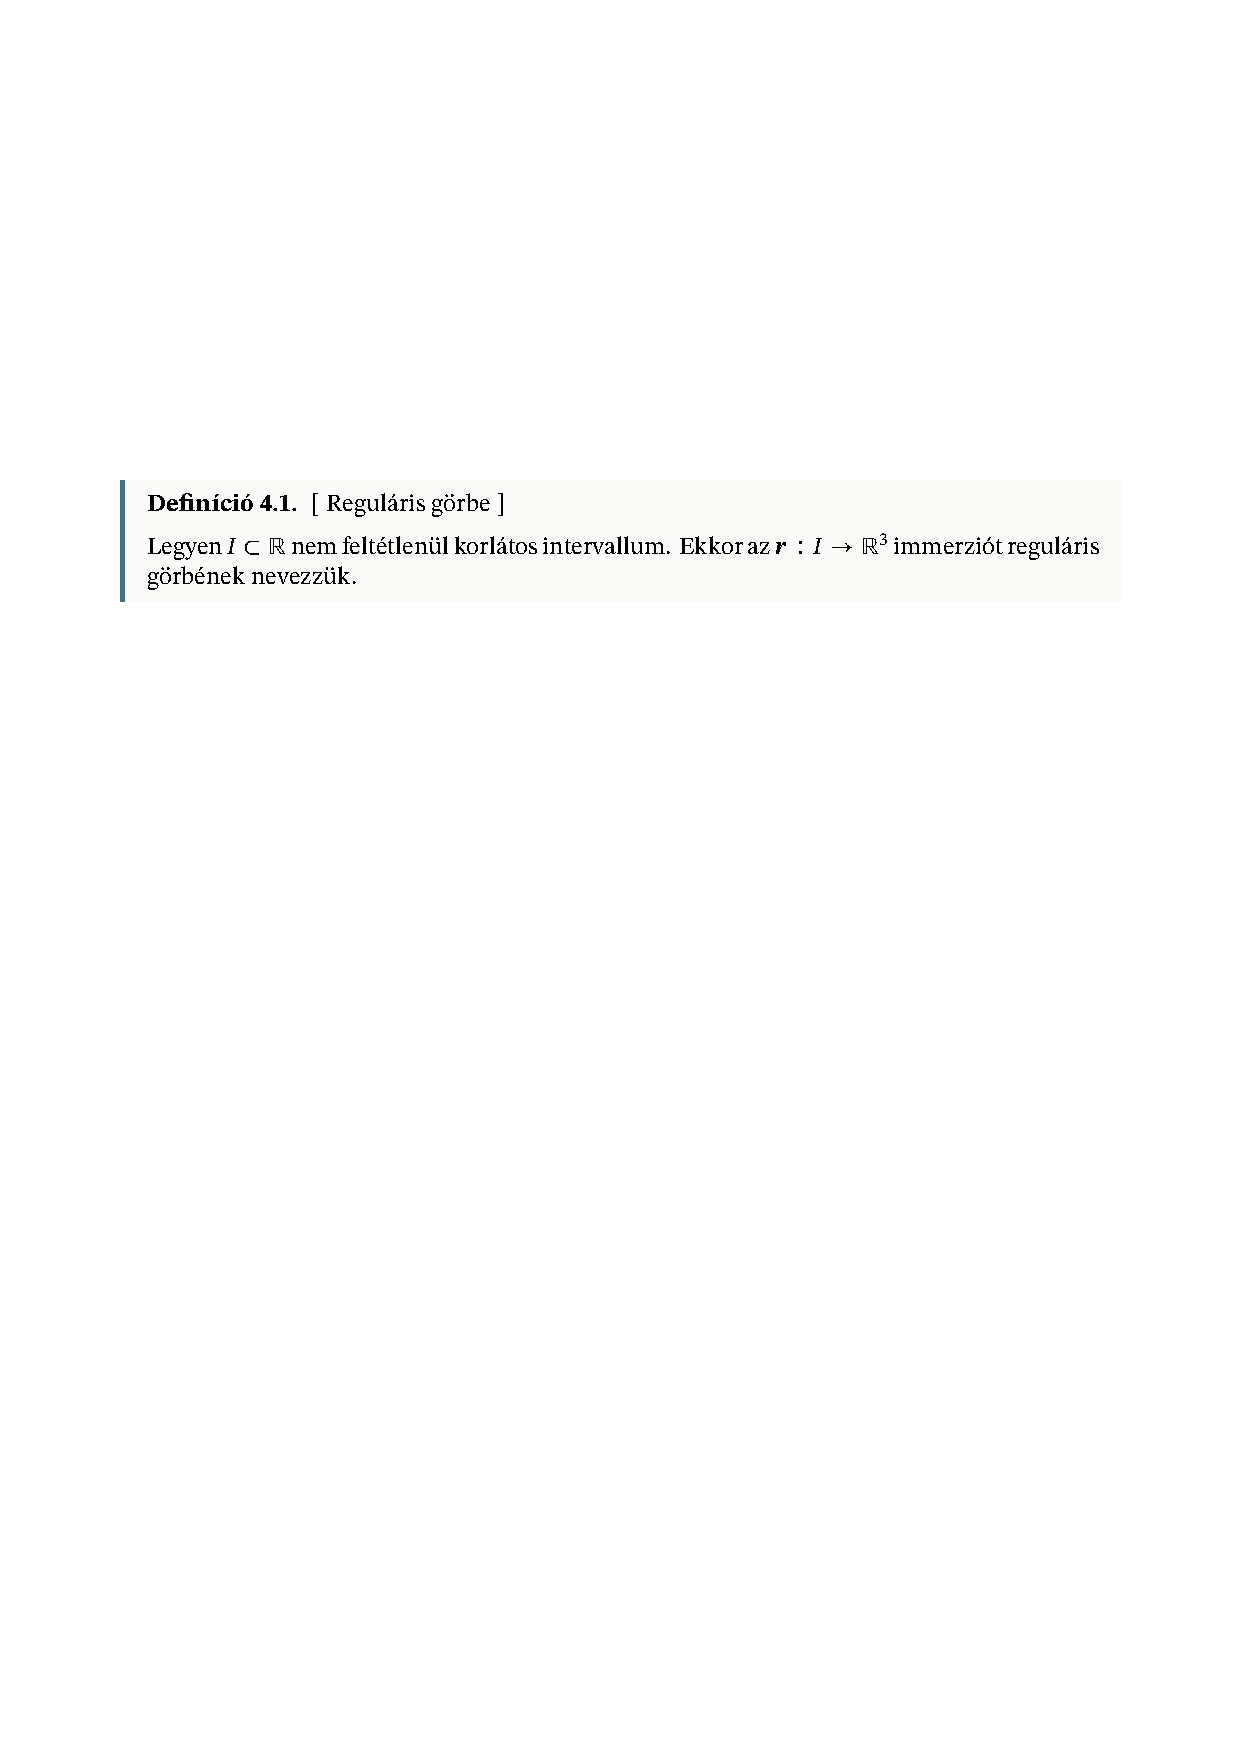
\includegraphics[width=\textwidth]{./figures/example-handout-definition.pdf}}
	}
	\caption{Egy definíció megjelenése}
\end{figure}

Az elmélet átismétlése után a hallgatók a gyakorló feladatokat találhatták meg.
Minden gyakorló anyag általában három feladatot tartalmazott, több alfeladattal
együtt. A szóban forgó iromány egy ívhossz számítós, egy skalármezős görbementi
integrálszámítós, és egy vektormezős görbementi integrálszámítós feladatot
tartalmaz, rendre négy, négy, és három alfeladattal.

\begin{figure}[htb]
	\centering
	{
		\setlength{\fboxsep}{10pt}%
		\setlength{\fboxrule}{2pt}%
		\renewcommand\fbox{\fcolorbox{gray}{white}}
		\fbox{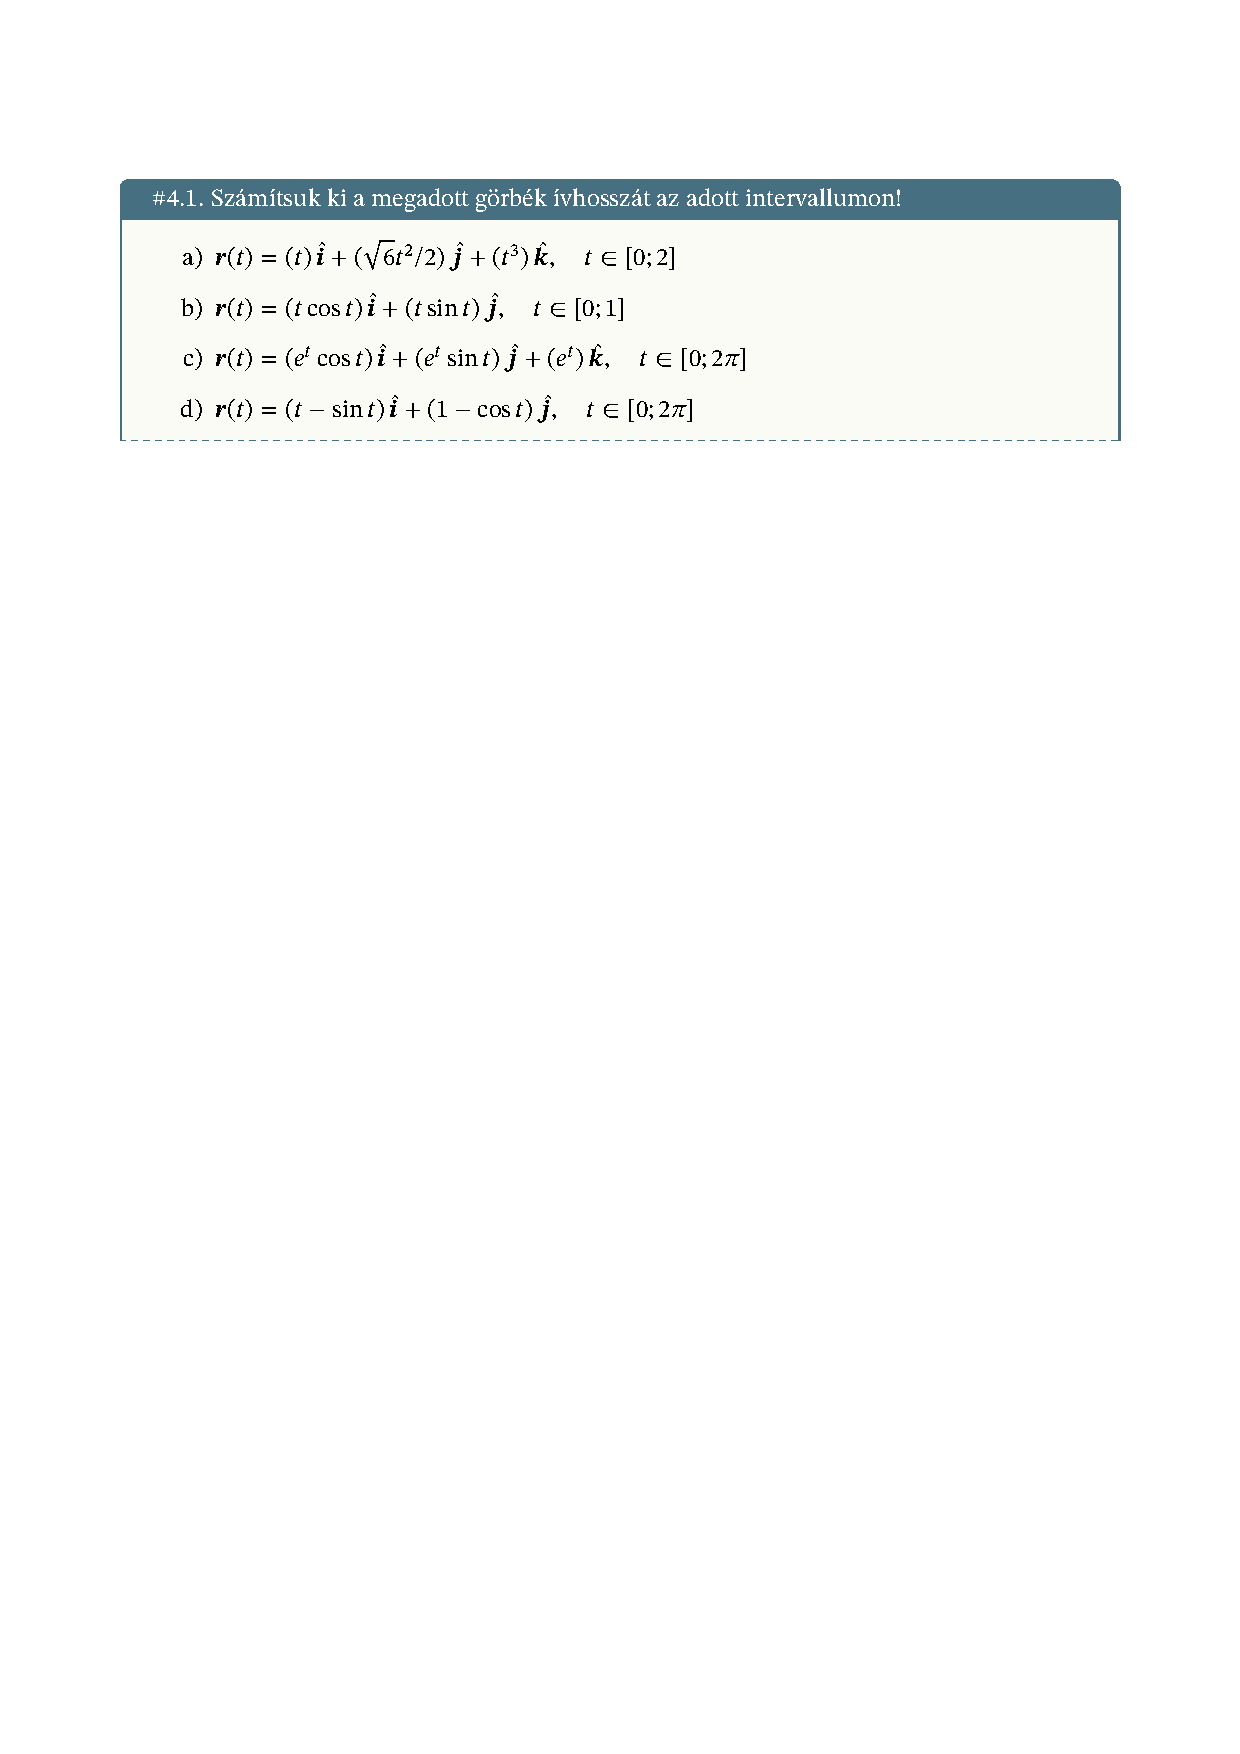
\includegraphics[width=\textwidth]{./figures/example-handout-exercise-no-sol.pdf}}
	}
	\caption{Görbe ívhosszának számítása}
\end{figure}

A feladatok kezelése a \texttt{math-exercise} csomagban definiált környezet
segítségével történt. A feladatok számozása automatikusan történt, előtagnak
pedig a dokumentum sorszámát használtam. A feladatok megoldásai is természetesen
elérhetőek voltak, a \texttt{math-handout} osztály a \texttt{math-exercise}
csomagot automatikusan a \texttt{print-solutions} paraméterrel hívja meg.

\begin{figure}[htb]
	\centering
	{
		\setlength{\fboxsep}{10pt}%
		\setlength{\fboxrule}{2pt}%
		\renewcommand\fbox{\fcolorbox{gray}{white}}
		\fbox{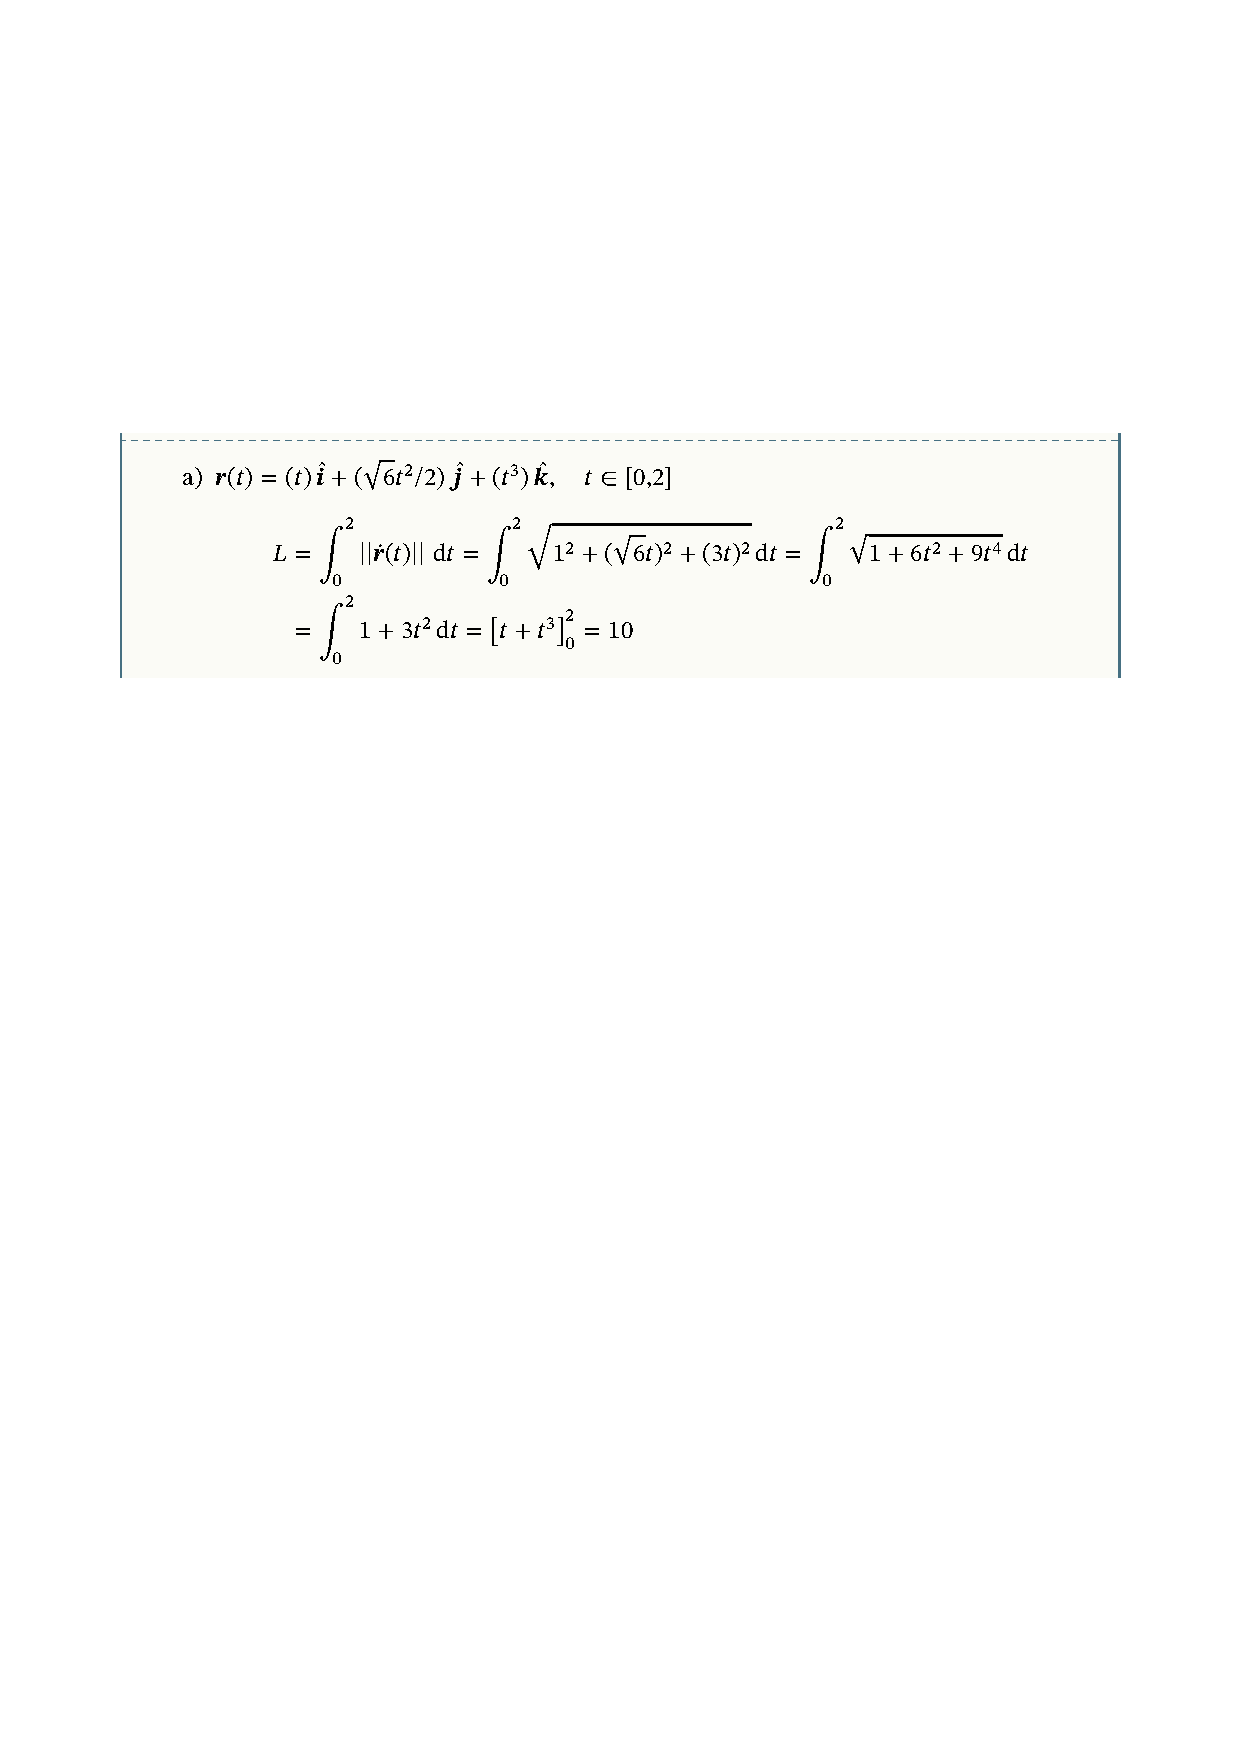
\includegraphics[width=\textwidth]{./figures/example-handout-exercise-just-sol.pdf}}
	}
	\caption{Az első alfeladat megoldása}
\end{figure}

A dokumentumok végén általában egy segédlet is található. Ez tartalmazhat
azonosságokat, vagy akár vizuális segítséget is nyújthat a hallgatóknak.
Ehhez a témakörhöz egy görbék paraméterezésével kapcsolatos összefoglalót
készítettem, amely tartalmazza a tantárgy során érintett legfontosabb görbék
paraméteres egyenleteit, és a hozzájuk tartozó ábrákat.

\begin{figure}[htb]
	\centering
	{
		\setlength{\fboxsep}{10pt}%
		\setlength{\fboxrule}{2pt}%
		\renewcommand\fbox{\fcolorbox{gray}{white}}
		\fbox{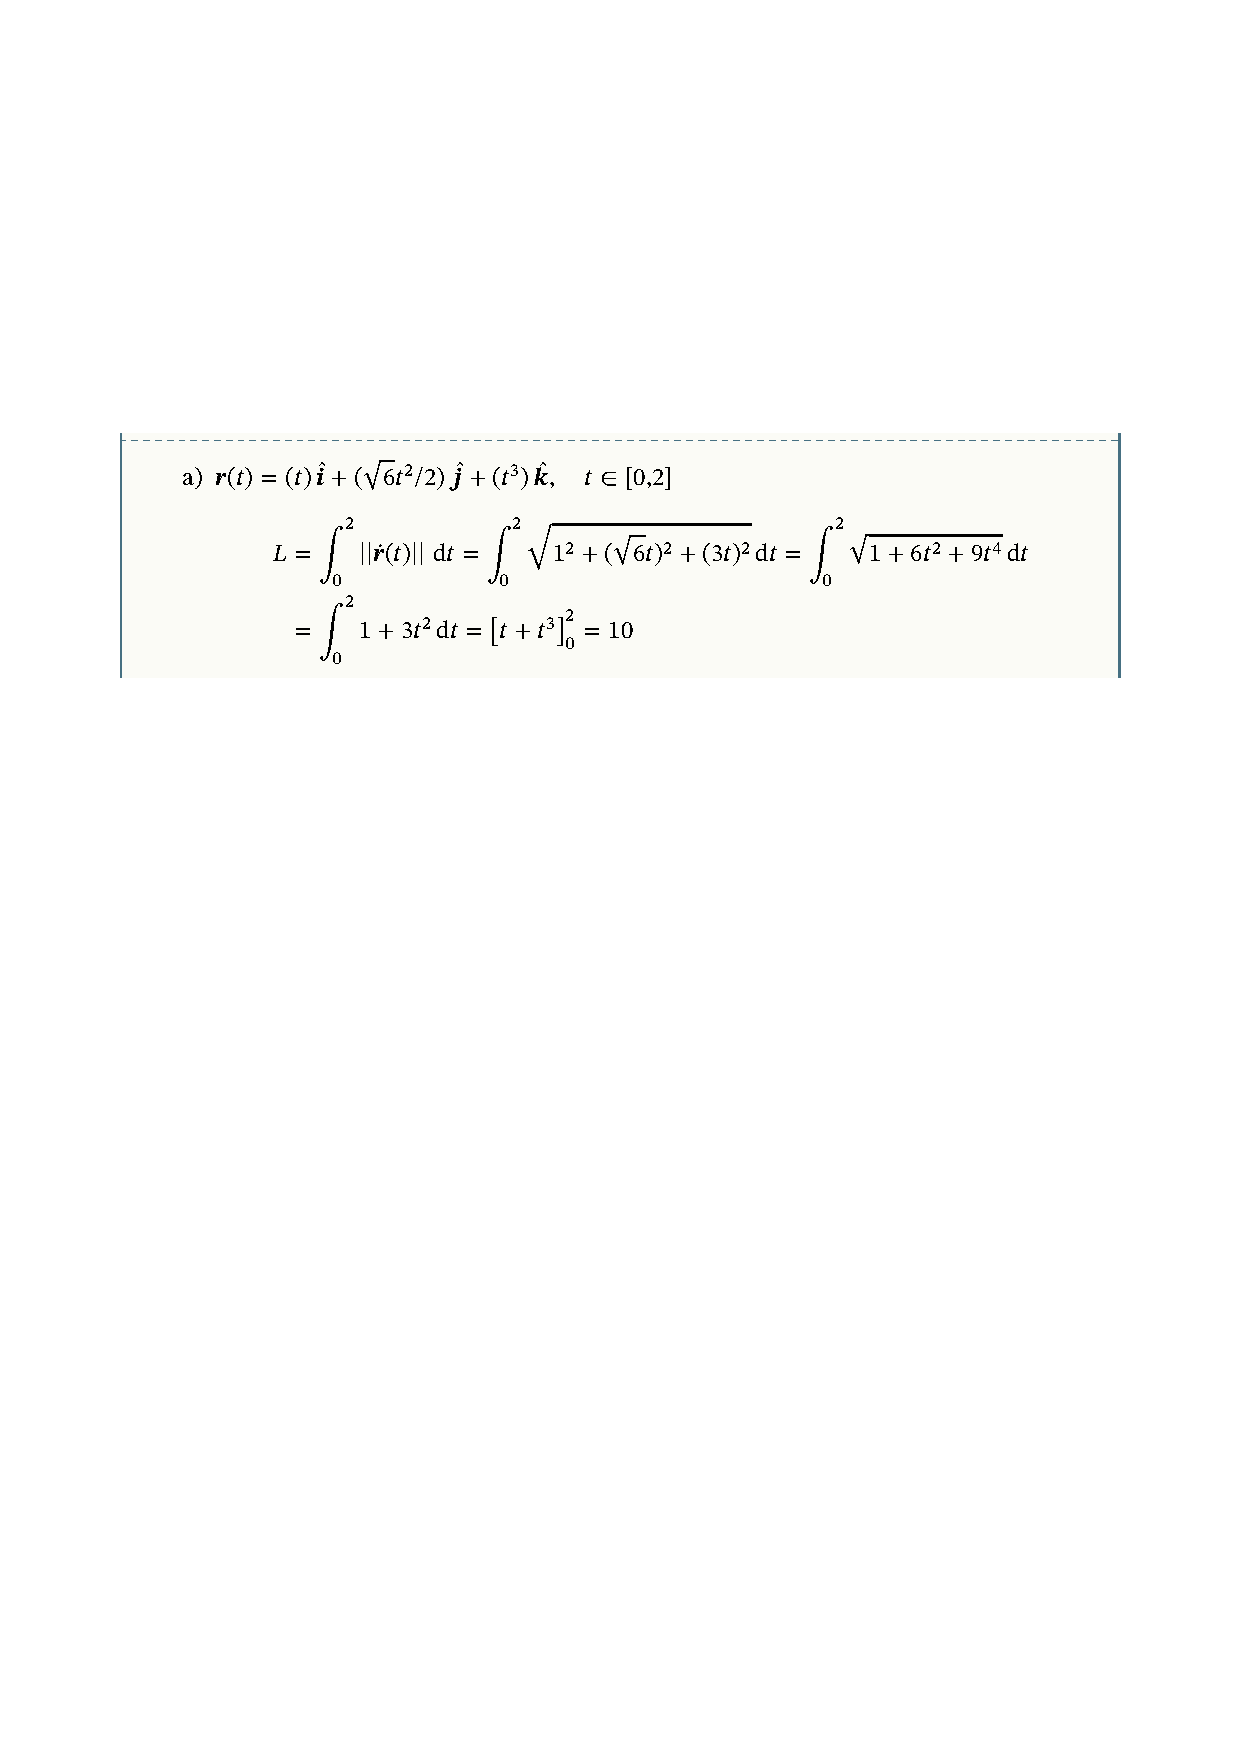
\includegraphics[width=\textwidth]{./figures/example-handout-exercise-just-sol.pdf}}
	}
	\caption{Egy $\mathbb R^3$-beli egyenes paraméterezése}
\end{figure}

% ------------------------------------------------------------------------------
\cleardoublepage
% ------------------------------------------------------------------------------
\chapter{A fejlesztői környezet bemutatása}
% ------------------------------------------------------------------------------

% Small introduction
Az oktatási anyagok bemutatása után térjünk át arra, hogy a projekt készítése
során milyen fejlesztői környezetben dolgoztam. Kitérek arra, hogy a
forrásfájlokat milyen környezetben tároltam, és hogy ez miért volt
elengedhetetlen egy ilyen nagy volumenű projekt menedzselése és
továbbfejleszthetősége érdekében. Ezután megmutatom, hogy milyen szkripteket
készítettem a hibák kiküszöbölése, a dokumentumok egyszerű fordítása érdekében,
valamint arra, hogy ezek a programok hogyan működnek a gyakorlatban.

% Ebben a fejezetben be fogom mutatni, hogy milyen környezetben dolgoztam a
% fejlesztés során. Kitérek arra, hogy a forrásfájlokat milyen környezetben
% tároltam. Megmutatom, hogy milyen szkripteket fejlesztettem, melyek
% elősegítették a hibák kiküszöbölését, a dokumentumok fordítását és a kódbázis
% bővítését is.

% ------------------------------------------------------------------------------
\section{Git: a verziókezelő rendszer}
% ------------------------------------------------------------------------------

% Git in general
A szoftverfejlesztés világában a \textit{git} rendszer egyre inkább alapvető
eszközzé válik. A \textit{git} nemcsak egy egyszerű verziókezelő rendszer,
hanem egy olyan eszköz is, amely újradefiniálja a fejlesztők munkamódszereit,
hiszen jelentős előnyöket nyújt a projektmenedzsment és a csapatmunka terén.

% ------------------------------------------------------------------------------
\subsection{Út a git megjelenéséig}
% ------------------------------------------------------------------------------

% Version control in general
Mi is az a verziókezelés, és miért is olyan fontos egy ilyen projekt esetén?
A verziókezelés egy olyan rendszer, amely lehetővé teszi, hogy egy adott
dokumentum, vagy fájl változásainak időben nyomon követését. Ezt a módszert
általában szoftverek forrásfájljainak nyilvántartására használják, de valójában
egy számítógépen található bármilyen típusú fájlra alkalmazható. Mivel jelen
esetben a fejlesztés során a forrásfájlok egyszerű szövegfájlok, ezért a
\textit{git} rendkívül hatékony eszköznek bizonyul.

% Copy paste
Sok embernél a verziókezelés abban merül ki, hogy a fájlokat egy másik
könyvtárba másolják, és a fájlok nevéhez egy sorszámot fűznek. Ez a megközelítés
rendkívül elterjedt, de sajnos nem túl hatékony, és még hibaérzékeny is. Könnyű
elfeledkezni arról, hogy melyik fájl melyik verzióját melyik könyvtárban
találhatjuk meg. Előfordulhat ezáltal, hogy egy régebbi verzióval dolgozunk,
vagy éppen egy másik fejlesztő munkáját írjuk felül.

\begin{figure}[htb]
	\centering
	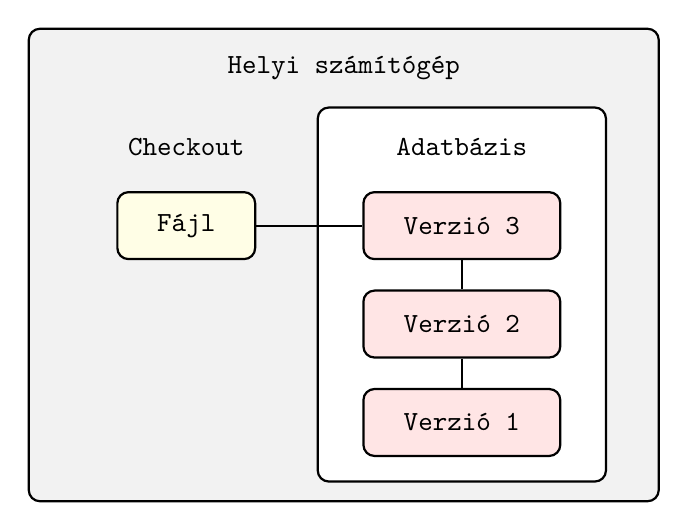
\begin{tikzpicture}[thick]
		\draw[rounded corners, fill=gray!10] (-4,-3) rectangle (4,3);
		\draw[rounded corners, fill=white] (-0.33,-2.75) rectangle (3.33,2);


		\node at (0, 2.5) {\texttt{Helyi számítógép}};

		\node at (-2,1.5) {\texttt{Checkout}};
		\node[
			rectangle, rounded corners, fill=yellow!10, draw=black,
			minimum width=1.75cm, minimum height=0.85cm
		] (F) at (-2,0.5) {\texttt{Fájl}};

		\node at (1.5, 1.5) {\texttt{Adatbázis}};

		\node[
			rectangle, rounded corners, fill=red!10, draw=black,
			minimum width=2.5cm, minimum height=0.85cm
		] (V3) at (1.5,0.5) {\texttt{Verzió 3}};
		\node[
			rectangle, rounded corners, fill=red!10, draw=black,
			minimum width=2.5cm, minimum height=0.85cm
		] (V2) at (1.5,-0.75) {\texttt{Verzió 2}};
		\node[
			rectangle, rounded corners, fill=red!10, draw=black,
			minimum width=2.5cm, minimum height=0.85cm
		] (V1) at (1.5,-2) {\texttt{Verzió 1}};

		\draw (F) -- (V3) -- (V2) -- (V1);
	\end{tikzpicture}
	\caption{Helyi verziókezelő rendszerek felépítése \cite{git_scm_1.1}}
	\label{fog:fig:local-vcs}
\end{figure}

% Local version control
Ennek a problémának az orvosolására a programozók már régen kifejlesztettek
helyi verziókezelő rendszereket, amelyek mögött egy egyszerű adatbázis állt.
Az egyik legnépszerűbb ilyen eszköz az \textit{RCS} (Revision Control System --
Revíziós Ellenőrzési Rendszer) volt, amely a mai napig számtalan \textit{Unix}
rendszeren elérhető. Az \textit{RCS} egy egyszerű rendszer, amely a fájlok
mentéséhez \textit{diff} fájlokat használ. A \textit{diff} fájlokban csak azok
a sorok szerepelnek, amelyek változtak, így ezen fájlok mérete kicsi marad.
\cite{rcs_documentation} Egy ilyen rendszer felépítése a
\ref{fog:fig:local-vcs}. ábrán látható.

\begin{figure}[htb]
	\centering
	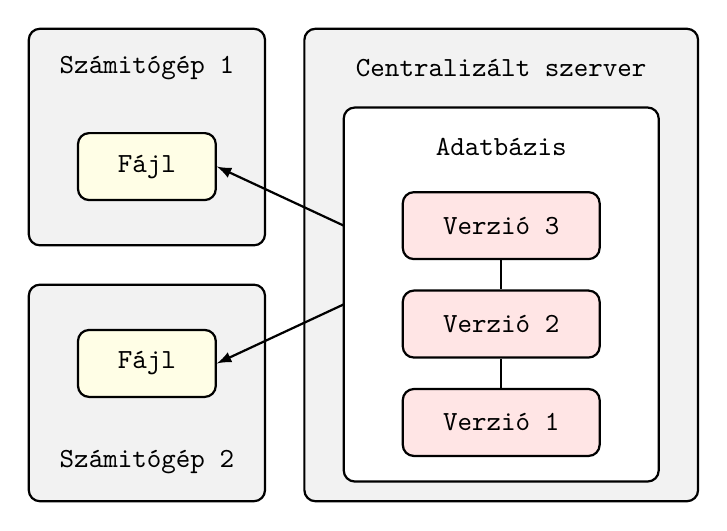
\begin{tikzpicture}[thick]
		\draw[rounded corners, fill=gray!10] (-4,-3) rectangle ++(3,2.75);
		\draw[rounded corners, fill=gray!10] (-4,0.25) rectangle ++(3,2.75);
		\draw[rounded corners, fill=gray!10] (-0.5,-3) rectangle ++(5,6);
		\draw[rounded corners, fill=white] (0,-2.75) rectangle (4,2);

		\node (C1) at (-2.5,2.5) {\texttt{Számitógép 1}};
		\node (C2) at (-2.5,-2.5) {\texttt{Számitógép 2}};

		\node[
			rectangle, rounded corners, fill=yellow!10, draw=black,
			minimum width=1.75cm, minimum height=0.85cm
		] (F1) at (-2.5,1.25) {\texttt{Fájl}};
		\node[
			rectangle, rounded corners, fill=yellow!10, draw=black,
			minimum width=1.75cm, minimum height=0.85cm
		] (F2) at (-2.5,-1.25) {\texttt{Fájl}};

		\node at (2,2.5) {\texttt{Centralizált szerver}};
		\node at (2, 1.5) {\texttt{Adatbázis}};

		\node[
			rectangle, rounded corners, fill=red!10, draw=black,
			minimum width=2.5cm, minimum height=0.85cm
		] (V3) at (2,0.5) {\texttt{Verzió 3}};
		\node[
			rectangle, rounded corners, fill=red!10, draw=black,
			minimum width=2.5cm, minimum height=0.85cm
		] (V2) at (2,-0.75) {\texttt{Verzió 2}};
		\node[
			rectangle, rounded corners, fill=red!10, draw=black,
			minimum width=2.5cm, minimum height=0.85cm
		] (V1) at (2,-2) {\texttt{Verzió 1}};

		\draw (V3) -- (V2) -- (V1);
		\draw [-latex] (0,.5) -- (F1.east);
		\draw [-latex] (0,-.5) -- (F2.east);
	\end{tikzpicture}
	\caption{Centralizált verziókezelő renszerek felépítése \cite{git_scm_1.1}}
	\label{fig:centralized-vcs}
\end{figure}

% Centralized version control
Az \textit{RCS} egy egyszerű, és hatékony rendszernek bizonyult, viszont volt
egy nagyon fontos hiányossága. A rendszer nem támogatta a többfejlesztői
munkát. Ennek a problémának az orvosolására fejlesztették ki a centralizált
verziókezelő rendszereket. Az ilyen rendszerek esetén (mint pl. a \textit{CVS}
(Concurrent Versions System -- Egyidejű verziók rendszere)) egy központi
szerver tárolja a fájlokat, és a fejlesztők a szerveren keresztül tudják
elérni a fájlokat. Egy ilyen rendszer használata számos előnnyel jár a helyi
rendszerekkel szemben, viszont van egy súlyos hibája, amely a központi
szerverben rejlik. Ha a szerver egy pár órára leáll, akkor senki sem tud
dolgozni. Ha a szerver a fájlokat tároló adathordozóval együtt elromlik,
az az adatok és történetük elvesztését jelenti. \cite{cvs_documentation}
Egy ilyen rendszer felépítése a \ref{fig:centralized-vcs}. ábrán látható.

\begin{figure}[htb]
	\centering
	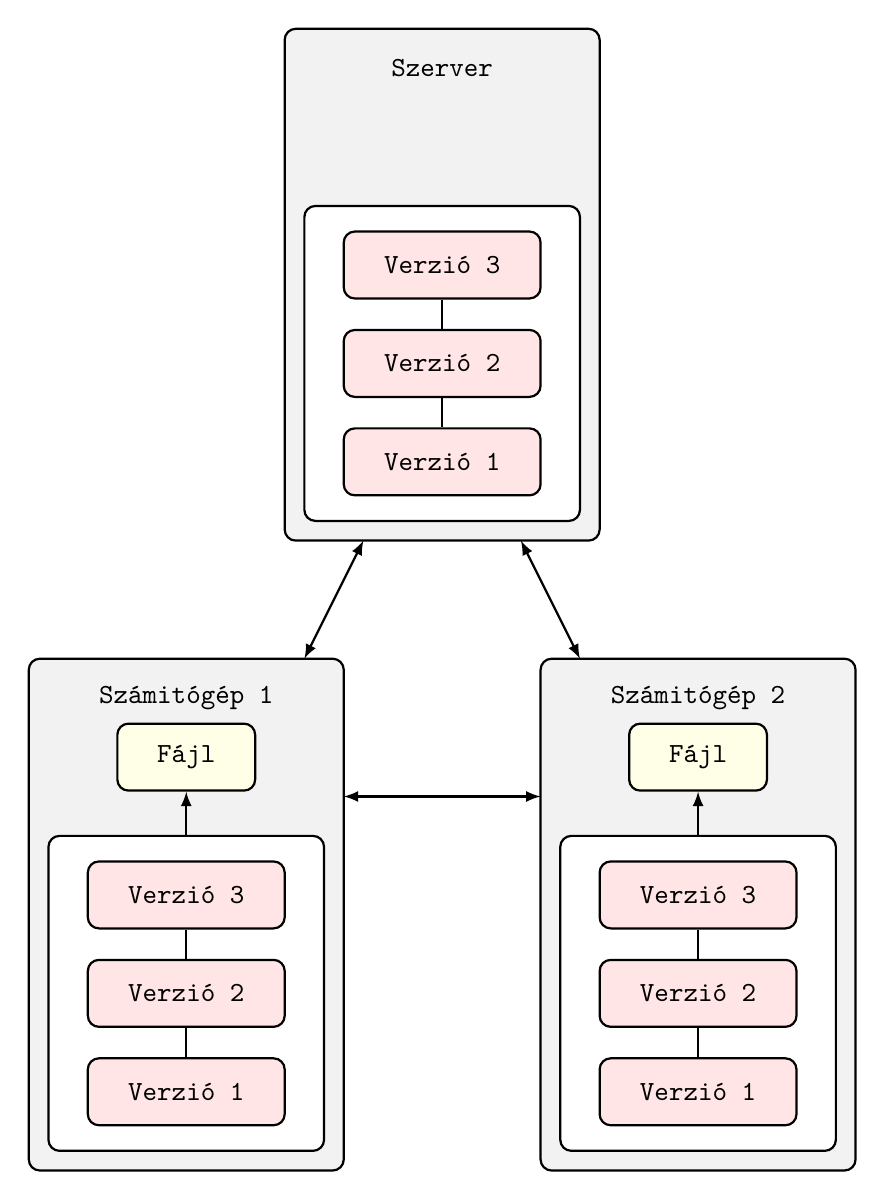
\begin{tikzpicture}[thick]
		\foreach \x/\y in {0/0,-1/-1,1/-1} {
				\begin{scope}[xshift=\x*3.25cm, yshift=\y*8cm]
					\draw[rounded corners, fill=gray!10] (2,3) rectangle ++(-4,-6.5);
					\draw[rounded corners, fill=white] (1.75,0.75) rectangle ++(-3.5,-4);

					\node[
						rectangle, rounded corners, fill=red!10, draw=black,
						minimum width=2.5cm, minimum height=0.85cm
					] (V3) at (0,0) {\texttt{Verzió 3}};
					\node[
						rectangle, rounded corners, fill=red!10, draw=black,
						minimum width=2.5cm, minimum height=0.85cm
					] (V2) at (0,-1.25) {\texttt{Verzió 2}};
					\node[
						rectangle, rounded corners, fill=red!10, draw=black,
						minimum width=2.5cm, minimum height=0.85cm
					] (V1) at (0,-2.5) {\texttt{Verzió 1}};

					\draw (V3) -- (V2) -- (V1);
				\end{scope}
			}

		\node (S) at (0,2.5) {\texttt{Szerver}};

		\node (C1) at (-3.25,-5.5) {\texttt{Számitógép 1}};
		\node (C2) at (3.25,-5.5) {\texttt{Számitógép 2}};
		\node[
			rectangle, rounded corners, fill=yellow!10, draw=black,
			minimum width=1.75cm, minimum height=0.85cm
		] (F1) at (-3.25,-6.25) {\texttt{Fájl}};
		\node[
			rectangle, rounded corners, fill=yellow!10, draw=black,
			minimum width=1.75cm, minimum height=0.85cm
		] (F2) at (3.25,-6.25) {\texttt{Fájl}};

		\draw [-latex] (-3.25,-7.25) -- (F1);
		\draw [-latex] (3.25,-7.25) -- (F2);

		\draw [latex-latex] (-1.25,-6.75) -- (1.25,-6.75);
		\draw [latex-latex] (-1.75,-5) -- (-1,-3.5);
		\draw [latex-latex] (1.75,-5) -- (1,-3.5);
	\end{tikzpicture}
	\caption{Centralizált verziókezelő renszerek felépítése \cite{git_scm_1.1}}
	\label{fig:distributed-vcs}
\end{figure}

% Distributed version control
Itt jönnek képbe a elosztott verziókezelő rendszerek, mint pl. a \textit{git}.
Ilyen rendszereknél a felhasználók nemcsak a fájlok legfrissebb verzióját
birtokolják, hanem teljes mértékben lemásolják az összes adatot, beleértve
a fájlokat, és azok teljes történetét is. Ez a megközelítés sokkal
biztonságosabb, mint a centralizált rendszereké, hiszen ha egy szerver
elromlik, akkor a fájlok másolatai még mindig elérhetőek. Ráadásul a legtöbb
ilyen rendszer jól kezeli, ha egy projekten belül több tárolóhelyet szeretnénk
használni. Ez a kedvező tulajdonság olyan munkafolyamatokat is lehetővé
tesz, amelyek centralizált rendszerekben nem megoldhatóak, például
hierarchikus modellek alkalmazását. \cite{git_scm_1.1} Egy ilyen verziókezelő
rendszer modellje a \ref{fig:distributed-vcs}. ábrán látható.

% ------------------------------------------------------------------------------
\subsection{A git rövid története}
% ------------------------------------------------------------------------------

% Git short history
A \textit{Linux kernel} egy nagyszabású, nyílt forráskódú projet. A kezdeti
időszakban a szoftver módosításait javítások és archivált fájlok formájában
terjesztették. 2002-ben a \textit{Linux kernel projekt} egy \textit{BitKeeper}
nevű, elosztott verziókezelő rendszerre tért át. 2005-ben a \textit{Linux}
fejlesztői és a \textit{BitKeeper} mögött álló cég közötti kapcsolat egyre
inkább leépült, a \textit{BitKeeper} szoftver ingyenes hozzáférése pedig
megszűnt. Ekkor a \textit{Linux} fejlesztői úgy döntöttek, hogy saját
verziókezelő rendszert fejlesztenek, amely a \textit{BitKeeper} által
használt adatmodellt követi. A projektet Linus Torvalds vezette, és a
\textit{git} nevet kapta. Az új rendszer készítése során az alábbi célokat
tartották szem előtt:
\begin{itemize}
	\item gyorsaság,
	\item egyszerűség,
	\item támogassa a nemlineáris fejlesztést,
	\item teljesen elosztott legyen,
	\item támogassa a nagy projekteket is
\end{itemize}
Az első megjelenés óta a \textit{git} nagyon sokat fejlődött, viszont a fenti
célok mindvégig megmaradtak, mára pedig a legelterjedtebb verziókezelő rendszer
lett. \cite{git_scm_1.2}

% ------------------------------------------------------------------------------
\subsection{Az alapok}
% ------------------------------------------------------------------------------

% Git basics
Egy \textit{git} alapú verziókezelő rendszer használata nagyon egyszerű.
Ha egy már meglévő projektet szeretnénk egy \textit{git} alapú rendszerbe
helyezni, akkor a következő parancsot kell kiadnunk:

\begin{lstlisting}[caption={A git inicializálása},language=sh]
  $ cd <projekt könyvtár> # A projekt könyvtárba navigálunk
  $ git init              # A projekt könyvtár verziókezelését inicializáljuk
\end{lstlisting}

A parancs hatására a könyvtárban létrejött egy \texttt{.git} nevű rejtett
mappa, amely tartalmazza a \textit{git} számára alapvető fájlokat.
Ezt a folyamatot a \textit{git repository} inicializálásának nevezzük.
Fontos, hogy ilyenkor a projetben található fájlok nem lesznek
automatikusan verziókezelve, hanem úgynevezett \texttt{untracked} állapotba
kerülnek. Ez azt jelenti, hogy a \textit{git} nem fogja nyomon követni a
fájlok változásait. Ahhoz, hogy egy fájlt a \textit{git} nyomon kövessen,
a következő parancsot kell kiadnunk:

\begin{lstlisting}[caption={Fájlok hozzáadása},language=sh]
  $ git add <fájl neve>
\end{lstlisting}

Ekkor a fájlok \texttt{staged} állapotba kerülnek, vagyis a következő
pillanatképbe bekerülnek. Ahhoz, hogy egy pillanatképet készítsünk a
projekt állapotáról, a következő parancsot kell kiadnunk:

\begin{lstlisting}[caption={Pillanatkép mentése},language=sh]
  $ git commit -m <A commit üzenet>
\end{lstlisting}

A parancs hatására a \textit{git} létrehoz egy pillanatképet a projekt
állapotáról, és a pillanatképhez hozzárendeli a megadott üzenetet. Az ebben
szereplő fájlok pedig \texttt{tracked}, vagyis nyomon követett állapotba
kerülnek. Amennyiben a fájlok módosulnak, úgy a \textit{git} automatikusan
\texttt{modified} állapotba helyezi őket. Ha a módosításokat menteni
szeretnénk, akkor a fenti parancsokat kell újra kiadnunk. A \texttt{git add}
parancs hatására a fájlok \texttt{staged} állapotba kerülnek, majd a
\texttt{git commit} parancs hatására a fájlok pillanatképe elkészül.
Az előbb leírt folyamatot a \ref{fig:git-lifecycle} ábra szemlélteti.

\begin{figure}[htb]
	\centering
	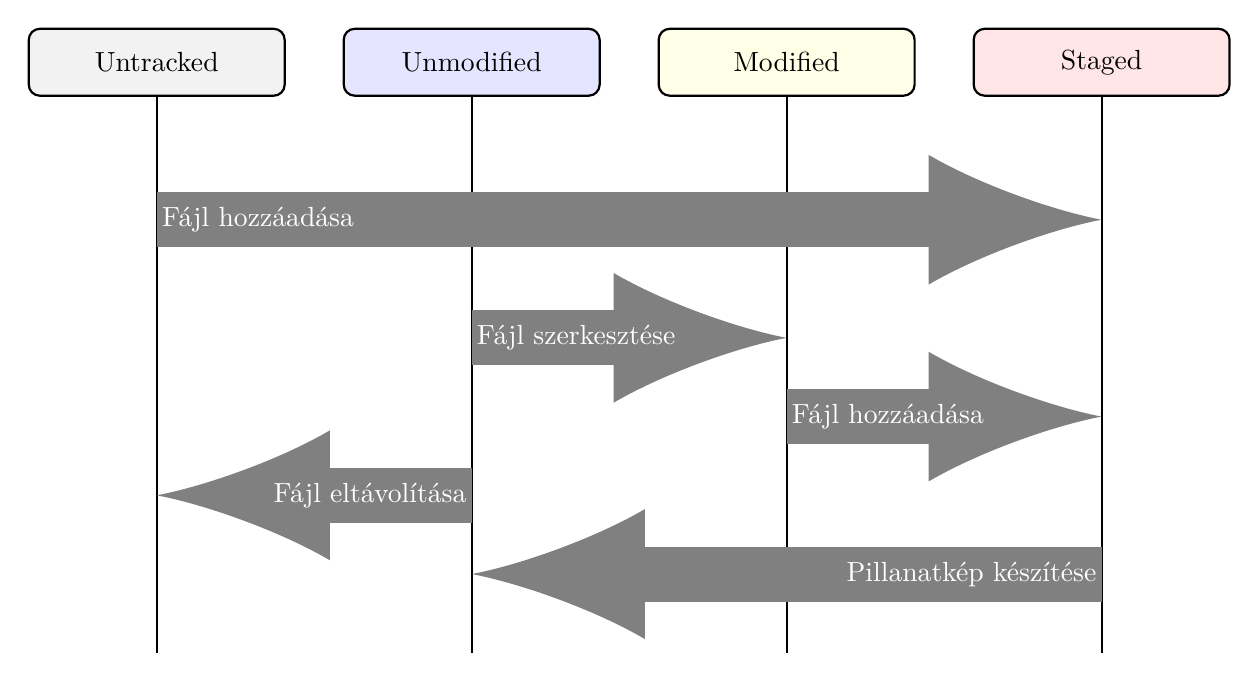
\begin{tikzpicture}[thick]
		\node[
			rectangle, rounded corners, fill=gray!10, draw=black,
			minimum width=3.25cm, minimum height=0.85cm
		] (U) at (-6, 0) {Untracked};
		\node[
			rectangle, rounded corners, fill=blue!10, draw=black,
			minimum width=3.25cm, minimum height=0.85cm
		] (X) at (-2, 0) {Unmodified};
		\node[
			rectangle, rounded corners, fill=yellow!10, draw=black,
			minimum width=3.25cm, minimum height=0.85cm
		] (M) at (2, 0) {Modified};
		\node[
			rectangle, rounded corners, fill=red!10, draw=black,
			minimum width=3.25cm, minimum height=0.85cm
		] (A) at (6, 0) {Staged};

		\foreach \l in {U,X,M,A} {
				\draw (\l) -- ++(0,-7.5);
			}

		\draw[-latex, line width=7mm, draw=gray] (-6,-2) -- (6,-2)
		node[right=-4mm, white, pos=0] {Fájl hozzáadása};
		\draw[-latex, line width=7mm, draw=gray] (-2,-3.5) -- (2,-3.5)
		node[right=-4mm, white, pos=0] {Fájl szerkesztése};
		\draw[-latex, line width=7mm, draw=gray] (2,-4.5) -- (6,-4.5)
		node[right=-4mm, white, pos=0] {Fájl hozzáadása};
		\draw[-latex, line width=7mm, draw=gray] (-2,-5.5) -- (-6,-5.5)
		node[left=-4mm, white, pos=0] {Fájl eltávolítása};
		\draw[-latex, line width=7mm, draw=gray] (6,-6.5) -- (-2,-6.5)
		node[left=-4mm, white, pos=0] {Pillanatkép készítése};
	\end{tikzpicture}
	\caption{%
		A fájlok életciklusa
		% Untracked -- Történet nélküli, újonnan létrehozott fájl\\
		% Unmodified -- A legutolsó pillanatkép óta nem módosított fájl\\
		% Modified -- A legutolsó pillanatkép óta módosított fájl\\
		% Staged -- Módosított, vagy újonnan létrehozott fájl,\\
		% \phantom{Staged -- }amely a következő pillanatképbe bekerül 
		\cite{git_scm_2.2}%
	}
	\label{fig:git-lifecycle}
\end{figure}

A fejlesztés során a programozók gyakran nem egyenként adják hozzá a fájlokat,
hanem a következő parancsot használják:

\begin{lstlisting}[caption={Összes fájl hozzáadása},language=sh]
  $ git add --all
\end{lstlisting}

A parancs hatására az összes újonnan létrehozott, vagy az utolsó pillanatkép
óta módosított fájl \texttt{staged} állapotba kerül. Ilyen parancsok
használata esetén nagyon hasznos tud lenni egy \texttt{.gitignore} nevű fájl.
Ez azoknak a fájloknak vagy almappáknak a listáját tartalmazza, amelyeket nem
szeretnénk, hogy a \textit{git} nyomon kövessen. Ilyen fájlok lehetnek pl. a
fordítóprogramok által generált fájlok és mappák (c program esetén a futtatható
állomány és az objektumfájlok), a fordítóprogramok által generált hibajelentések
(\textit{gcc} esetén a \texttt{.o} és \texttt{.out} fájlok, vagy akár az
operációs rendszer által generált rejtett fájlok (\textit{MacOS}-en a
\texttt{.DS\_Store},  \textit{Windows}-on a \texttt{Thumbs.db} fájlok).
Az én projektemben ez a fájl majdnem 500 sor hosszú, a legfontosabb elemei
a következőek:
\begin{lstlisting}[caption={A projektemben található \texttt{.gitignore} fájl legfontosabb részei},language=sh]
  # Projekt specifikus
  build     # A latexmk által generált fájlok
  generate  # A tsc által generált fájlok
  *.log     # A formázóprogramok és az automatizáló szkriptek által generált fájlok

  # Operációs rendszer specifikus
  .DS_Store
\end{lstlisting}

% ------------------------------------------------------------------------------
% \subsection{A git repositoryk kezelése}
% ------------------------------------------------------------------------------

% Ahhoz, hogy egy projekten több fejlesztő tudjon együtt dolgozni, tudnunk
% kell kezelni az úgynevezett \textit{remote repository}-kat. Ezeket a
% \textit{repository}-kat általában az interneten, vagy helyi hálózaton
% tárolják. 

% ------------------------------------------------------------------------------
\section{Az automatizálás}
% ------------------------------------------------------------------------------

A fejlesztés során a \textit{git} mellett nagy segítségemre voltak az
automatizáló szkriptek. Ebben a szekcióban bemutatom, hogy milyen nyelvet
használtam a szkriptek írásához, és hogy ezek milyen feladatokat láttak el.

% ------------------------------------------------------------------------------
\subsection{A TypeScript nyelv}
% ------------------------------------------------------------------------------

A szkriptek létrehozása során mindenképpen egy olyan nyelvet szerettem volna
használni, amelyet már ismerek, és amely alkalmas a feladatok elvégzésére.
Fontos szempont volt az is, hogy bármilyen operációs rendszeren és a
\textit{Github Actions} környezetben is működjön. A választásom a
\textit{TypeScript} nyelvre esett, amely egy \textit{Microsoft} által
fejlesztett, nyílt forráskódú nyelv. Célja, hogy a \textit{JavaScript} nyelvhez
képest több lehetőséget biztosítson a programozók számára. Emiatt a fejlesztők
körében nagyon népszerű. A \textit{Stack Overflow} 2023-as felmérése szerint
a nyelv a harmadik legkelendőbb a piacon. A fejlesztők közel $72\%$-a azt
nyilatkozta, hogy szívesen használná a nyelvet a következő évben is.
\cite{SO_Survey_2023} Ez az eredmény nem meglepő, a nyelv ugyanis számos
előnnyel rendelkezik, amelyek közül a legfontosabbak a következőek:
\begin{enumerate}
	\item \textbf{Statikus típusosság és típusellenőrzés}:
	      A \textit{JavaScripttel} ellentétben a \textit{TypeScript} egy erősen
	      típusos nyelv. Ez azt jelenti, hogy lehetővé teszi változók,
	      függvényparaméterek és visszatérési értékek típusának fejlesztés közben
	      történő meghatározását, csökkentve a futási időben jelentkező
	      típushibákat.

	\item \textbf{Átlátható és karbantartható kód}:
	      Mivel a kód expliciten meghatározott típusokat és interfészeket
	      tartalmaz, ezért a kód könnyebb olvasható és karbantartható.
	      Ez különösen nagy projektek esetén jelenthet előnyt.

	\item \textbf{Kiváló fejlesztési eszközök}:
	      A \textit{TypeScript} nyelvhez kiváló fejlesztési eszközök állnak
	      rendelkezésre, melyek hatékonyabbá teszik a fejlesztést. A
	      legnépszerűbb szövegszerkesztők mind támogatják a nyelvet, a kód
	      automatikus formázásától kezdve a hibák jelzéséig. A legnépszerűbb
	      fejlesztői környezetek, mint pl. a \textit{Visual Studio Code} és
	      a \textit{WebStorm} pedig kifejezetten a \textit{TypeScript}
	      nyelvhez készültek.

	\item \textbf{Kompatibilitás és teljesítmény}:
	      A \textit{TypeScript} nyelv kódját a fordító program \textit{JavaScript}
	      kóddá fordítja, így a nyelvvel írt programok bármelyik
	      \textit{JavaScript} környezetben futtathatóak, teljesítményük
	      pedig azonos a \textit{JavaScript} nyelvű programokéval. Ráadásul egy
	      már meglévő \textit{JavaScript}-tel írt projekthez fokozatosan hozzá
	      lehet adni a \textit{TypeScript} nyelvű fájlokat, nem kell az egészet
	      újraírni.

	\item \textbf{Kiváló dokumentáció és támogatás}:
	      A programozók részére rendkívül fontos, hogy egy nyelv jól dokumentált
	      legyen. A \textit{TypeScript} nyelv fejlesztői a hivatalos dokumentáció
	      \cite{TS_Microsoft} mellett a \textit{Mozilla} által fenntartott
	      \textit{MDN Web Docs} \cite{JS_Mozilla} oldalon is választ találhatnak
	      a kérdéseikre.
\end{enumerate}

% ------------------------------------------------------------------------------
\subsection{A szkriptek működése}
% ------------------------------------------------------------------------------

% General description
A szkripteknek két fő feladata volt a fejlesztés során. Az első a dokumentumok
validálása, a második pedig a dokumentumok fordítása és rendszerezése volt.

% ------------------------------------------------------------------------------
\subsubsection{A projektstruktúra megtervezése}
% ------------------------------------------------------------------------------

% Folder structure
Első lépés a projektstruktúra megtervezése volt. A projekt gyökerében nyolc
fontos mappa, valamint konfigurációs fájlok találhatóak. Előbbiek közül öt
könyvtár \LaTeX, egy \textit{git}, egy \textit{TypeScript}, egy pedig
\textit{Github} specifikus volt. A konfigurációs fájlok egyrészt formázási
szabályokat, másrészt fordítási beállításokat tartalmaztak. Előbbiek használata
egy verziókezelő rendszerben nagyon fontos, hiszen így biztosítható, hogy minden
fejlesztő ugyanolyan formázási szabályokkal szerkesztett dokumentumokat
produkáljon. Ez \LaTeX esetében az \texttt{indentconfig.yaml},
\textit{TypeScript} esetében pedig a \texttt{.prettierrc} fájlt takarja.
A forditási beállításokat tartalmazó fájlok pedig a \texttt{.latexmkrc} és a
\texttt{tsconfig.json} fájlok voltak. A mappastruktúra a következőképpen
nézett ki:

\begin{lstlisting}
  │
  ├── .git     -- git specifikus fájlok
  ├── .github  -- github specifikus fájlok
  ├── scripts  -- Typescript files - only used in workflows
  │
  ├── config   -- LaTeX - osztályok és csomagok forrásai
  ├── book     -- LaTeX - math-book osztállyal készített dokumentumok
  ├── handout  -- LaTeX - math-handout osztállyal készített dokumentumok
  ├── exercise -- LaTeX - math-standalone osztállyal készített feladatok
  └── graphics -- LaTeX - math-standalone osztállyal készített ábrák
\end{lstlisting}

% ------------------------------------------------------------------------------
\subsubsection{A fájlkonvenció megtervezése}
% ------------------------------------------------------------------------------

% File convention
A mappastruktúra megtervezése után fontos volt további döntéseket hozni.
Be kellett vezetni egy nevezéktanbeli konvenciót, hogy a szkriptek könnyedén
megtalálják a dokumentumok forrásfájljait. Ennek érdekében minden mappába,
ahol úgynevezett gyökér fájlok voltak, egy \texttt{config.yml} fájlt kell
elhelyezni. Fontos, hogy amennyiben a program egy mappában egy ilyen
konfigurációs fájlt talál, akkor az alatta lévő mappákban már nem fog
tovább keresni. Például ha a \texttt{/handout/G3/multivariable} mappában
található egy \texttt{config.yml} fájl, akkor a program nem fogja
megvizsgálni a \texttt{/handout/G3/multivariable/1} mappát.

Egy \texttt{config.yml} fájl az alábbi kulcs-érték párokat tartalmazhatja:

\begin{lstlisting}[caption={A konfigurációs fájlok sémájának interfésze \textit{TypeScript} nyelvben}]
  interface LatexConfig {
    root_files: {
      input: string;
      output?: string;
      lang?: string;
    }[];
    lang?: string | boolean;
    external_deps?: {
      [key: string]: string[];
    };
  }
\end{lstlisting}

% root_files
Az egyetlen kötelező kulcs a \texttt{root\_files}, amely egy olyan objektumokból
álló tömb, melyek tartalmazzák a gyökér fájlok nevét (\texttt{input}),
opcionálisan pedig a kimeneti fájl nevét (\texttt{output}), és a dokumentum
nyelvét is (\texttt{lang}). A többi kulcs opcionális.

% lang
A \texttt{lang} kulcs alapértelmezett értéke a \texttt{true}, amely azt jelenti,
hogy amennyiben a dokumentum neve mellett nem adtuk meg a dokumentum nyelvét,
akkor a szkript a fájl elnevezése alapján fog következtetni annak nyelvére.
Magyar nyelvű fájlok esetén a \texttt{.hu.tex}, angol nyelvű fájlok esetén
pedig a \texttt{.en.tex} kiterjesztés jelzi a dokumentum nyelvét. Amennyiben
a fájl elnevezése nem a konvenció szerint történt, akkor a szkript egy
figyelmeztető üzenetet fog kiírni, de a fordítást nem fogja megállítani.
Ha az értéke \texttt{false}, az azt jelenti, hogy az adott mappában található
fájlok nem nyelv specifikusak. Ez az opció az ábráknál hasznos, hiszen azok
általában nem tartalmaznak szöveget. Megadhatjuk még a \texttt{lang} kulcsnak
egy nyelvkódot is. Ekkor a program nem fogja figyelembe venni a fájl nevét,
hanem minden fájlt a megadott nyelvűnek fogja tekinteni. Ha a dokumentum neve
mellett a nyelv kulcsot is tartalmazza a \texttt{root\_files} tömbben
található objektum, akkor az az érték felül fogja írni a \texttt{lang} kulcs
értékét.

% external_deps
A \texttt{external\_deps} kulcs pedig egy olyan objektumot tartalmaz, amely
úgynevezett külső programok csomagjaira mutat. Ezeket a szkript fordítás előtt
automatikusan telepíti annak érdekében, hogy a fordítás sikeres legyen. Például
ha megadjuk a \texttt{python} kulcsot, mely értéke:
\inlinecode{["numpy", "sympy"]},
akkor a szkript a fordítás előtt automatikusan telepíti a \textit{numpy} és a
\textit{sympy} csomagokat. Jelen esetben ez a funkció egyedül a
\textit{python} nyelv esetén érhető el, viszont más nyelvekre is könnyedén
kiterjeszthető a moduláris felépítésnek köszönhetően. Ez a funkció
különösen hasznos a \textit{Github Actions} környezetben, melyet a későbbiekben
fogok bemutatni.

% ------------------------------------------------------------------------------
\subsubsection{A szkriptek futtatása és kimenete}
% ------------------------------------------------------------------------------

A projekt gyökerében található egy \texttt{package.json} fájl, amelyben
különböző parancsokat definiáltam. Az alábbi opciók állnak rendelkezésre:

\begin{itemize}
	\item \textbf{\texttt{link}}:
	      Az osztályok és csomagok linkelése a \texttt{texmf} mappába.
	      Hatására a projektben szereplő összes \LaTeX{} osztály és csomag
	      elérhetővé válik a \LaTeX fordítóprogram számára. A gyakorlatban
	      ez azt jelenti, hogy a \texttt{config} mappában található osztályok
	      és csomagok hard linkelve -- vagy ha ez nem elérhető akkor másolva --
	      lesznek a \texttt{texmf} mappába, amely nemcsak a fordítónak,
	      hanem a fejlesztést segítő \LaTeX{} nyelvi szervernek is
	      esszenciális. Így a gyári csomagokhoz hasonlóan a saját forrásfájlokban
	      definiált parancsok is automatikusan felismerésre kerülnek.

	\item \textbf{\texttt{clean}}:
	      Kitörli a fordítás során keletkezett fájlokat.

	\item \textbf{\texttt{generate}}:
	      Elkészíti a fordítás során szükséges \texttt{shell scripteket}

	\item \textbf{\texttt{deps:<root|standalone|all>}}:
	      Installálja a külső függőségeket. A \texttt{root} csak a könyv és
	      handout osztályokhoz tartozó, a \texttt{standalone} csak a
	      \texttt{standalone} osztályokhoz tartozó, az \texttt{all} pedig
	      az összes fájlhoz tartozó dependenciákat telepíti.

	\item \textbf{\texttt{compile:<root|standalone|all>}}:
	      Elkészíti a dokumentumokat. A \texttt{root} csak a könyv és
	      handout osztályokhoz tartozó, a \texttt{standalone} csak a
	      \texttt{standalone} osztályokhoz tartozó, az \texttt{all} pedig
	      az összes fájlt lefordítja.
\end{itemize}

A fenti parancsokat a \texttt{pnpm} csomagkezelő segítségével lehet futtatni.
Ehhez lokálisan telepített \texttt{node} környezet szükséges. Mivel ennek a
\texttt{pnpm} alapértelmezetten nem része, ezért ennek telepítése is szükséges.
Ennek installálása, majd a fenti parancsok futtatása a következőképpen történik:
\begin{lstlisting}[caption={A pnpm telepítése és a parancsok futtatása}]
  $ npm install -g pnpm         # A pnpm telepítése
  $ pnpm run <parancs neve>     # A parancsok futtatása
\end{lstlisting}

% ------------------------------------------------------------------------------
\section{A projekt publikálása}
% ------------------------------------------------------------------------------

% General info
A szkriptek, bár egyértelműen hasznosak voltak a lokális fejlesztés során is,
hiszen a dokumentumok fordítását és validálását automatizálták, fő céljuk
mégsem ez volt. A projekt a \textit{Github} nevezetű platformon lett tárolva,
amely automatizálási lehetőségeket is biztosít. Ezt a lehetőséget kihasználva
a szkripteket a \textit{Github Actions} környezetben futtattam, ahol
a dokumentumok fordítása és validálása automatikusan megtörtént. Ennek a
folyamatát fogom most bemutatni.


% ------------------------------------------------------------------------------
\subsection{A Github}
% ------------------------------------------------------------------------------

% Github
A \textit{GitHub} egy -- egy \textit{Microsoft} által fejlesztett --
verziókezelésre és közös szoftverfejlesztésre tervezett webes platform, amely
a Linus Torvalds által létrehozott \textit{git} verziókezelő rendszerre épül.
Rendkívül népszerű a nyílt forráskódú projektek körében, felhasználói bázisa
2023-ra elérte a 100 millió főt. \cite{github_user_count}

A \textit{Github} rendkívül részletes dokumentációt, oktatási anyagokat és
fórumokat biztosít a felhasználói számára, ezért használatának elsajátítása
rendkívül egyszerű, és hasznos tud lenni a fejlesztés során.
\cite{github_documentation}

% ------------------------------------------------------------------------------
\subsection{A Github Actions}
% ------------------------------------------------------------------------------

% Github Actions
A \textit{Github Actions} egy olyan szolgáltatás a \textit{Github} platformon
belül, amely a felhasználók számára lehetővé teszi automatizálási folyamatok
hozzáadását a projektjeikhez. Használata nyílt forráskódú projektek esetén
korlátlanul ingyenes. Ez a képesség jelentősen kiterjeszti a \textit{Github}
funkcióit a puszta verzíókezelésen túl.

A \textit{Github Actions} segítségével olyan munkafolyamatok hozhatóak létre,
mint például a csomagok tesztelése, a hibák észlelése, vagy éppen kód fordítása,
vagy megjelentetése. Ezeket a folyamatokat úgynevezett \texttt{workflow}
fájlokban lehet definiálni, melyek a \texttt{/.github/workflows} mappában
található, \texttt{.yaml} kiterjesztésű fájlok.

Az általam létrehozott \texttt{workflow} fájlnak három fő része van. Az első
részben a fordításhoz szükséges \texttt{shell szkriptek} generálása történik.
Ez a folyamat a következőképpen néz ki:

\begin{enumerate}
	\item \textbf{\texttt{actions/checkout}}:
	      A projekt klónozása a szerverre.

	\item \textbf{\texttt{actions/setup-node}}:
	      A \texttt{node} környezetet telepítése.

	\item \textbf{\texttt{pnpm/action-setu}}:
	      A \texttt{pnpm} csomagkezelő telepítése.

	\item \textbf{\texttt{cache-dirs}}:
	      A \texttt{pnpm} cache mappája útvonalának eltárolása.

	\item \textbf{\texttt{actions/cache}}:
	      A \texttt{pnpm} cache mappájának elmentése. Ez a funkció azért hasznos,
	      mert amennyiben a fejlesztés a \texttt{package.json} fájlban megadott
	      dependenciák nem változnak, akkor a \texttt{pnpm} nem fogja újra
	      telepíteni őket, hanem a cache mappából fogja őket betölteni.
	      Ezzel a munkafolyamattal az inicializálás ideje jelentősen csökken.

	\item \textbf{\texttt{pnpm-deps}}:
	      Külső dependenciák telepítése. A \texttt{pnpm} csomagkezelő ebben a
	      lépésben telepíti a \texttt{package.json} fájlban definiált
	      dependenciákat.

	\item \textbf{\texttt{pnpm-generate}}:
	      A \texttt{shell szkriptek} generálása. A \texttt{pnpm} csomagkezelő
	      ebben a lépésben generálja a \texttt{shell szkripteket}, amelyek
	      a dokumentumok fordításához szükségesek.

	\item \textbf{\texttt{actions/upload-artifact}}:
	      A generált szkriptek eltárolása annak érdekében, hogy azok a következő
	      munkafolyamatban is elérhetőek legyenek.
\end{enumerate}

Miután a fordításhoz szükséges szkriptek sikeresen elkészültek, megkezdődik
a másik kettő folyamat, amelyek párhuzamosan futnak. Az egyik a könyv és
handout, a másik pedig a feladat és grafika típusú fájlok fordítását és
megjelentetését végzi el. Utóbbi inkább fejlesztési szempontból fontos, mivel
az ezekben található fájlok a könyvekben, illetve handoutokban szereplő
feladatokat és ábrákat tartalmazzák. A két folyamat felépítése teljesen azonos,
csupán abban tér el, hogy milyen típusú fájlokat dolgoznak fel:

\begin{enumerate}
	\item \texttt{\textbf{actions/checkout}}:
	      Az előzőekhez hasonlóan a projekt klónozása a szerverre.

	\item \texttt{\textbf{get-date}}:
	      A jelenlegi dátum eltárolása.

	\item \texttt{\textbf{actions/cache}}:
	      A generált fájlok elmentése. Amennyiben a fájlok nem változtak, akkor
	      nem kell újra lefordítani őket, ezzel drasztikusan lecsökkentve a
	      futási időt.

	\item \texttt{\textbf{actions/download-artifact}}:
	      A korábban generált szkriptek letöltése.

	\item \texttt{\textbf{link}}:
	      Az általam készített osztályok és csomagok másolása a \texttt{texmf}
	      mappába.

	\item \texttt{\textbf{dependencies}}:
	      A külső dependenciák telepítése.

	\item \texttt{\textbf{compile}}:
	      A dokumentumok fordítása.

	\item \texttt{\textbf{actions/upload-artifact}}:
	      A fordítás során keletkezett fájlok feltöltése.
\end{enumerate}

% ------------------------------------------------------------------------------
\cleardoublepage
% ------------------------------------------------------------------------------
\chapter{Tanuláselmélet}
% ------------------------------------------------------------------------------

%-------------------------------------------------------------------------------
\chapter{\osszefoglalas} % (Eredmények értékelése)
%-------------------------------------------------------------------------------

\section{Eredmények}

\begin{center}
	\Huge
	TODO: RESULTS
\end{center}


\section{Javaslatok/Következtetések/Tanulságok}

\begin{center}
	\Huge
	TODO: CONCLUSIONS/RECOMMENDATIONS/LESSONS LEARNED
\end{center}

\vspace{0.5cm}

\begin{flushleft}
	{Budapest, \today}
\end{flushleft}

\begin{flushright}
	\emph{\authorName}
\end{flushright}

\vfill

% Main content ends here

\addcontentsline{toc}{chapter}{\bibname}{%
	\footnotesize%
	\bibliography{bib/mybib}
}

%-------------------------------------------------------------------------------
\chapter*{\summary}\addcontentsline{toc}{chapter}{\summary}
%-------------------------------------------------------------------------------

\selectforeignlanguage % angol (magyar) nyelvi beállítások

Summary in English.

% \vspace{0.5cm}
% \paragraph{Keywords} \emph{\keywords}

\selectthesislanguage

%-------------------------------------------------------------------------------
\appendix
%-------------------------------------------------------------------------------
\chapter*{\fuggelek}\addcontentsline{toc}{chapter}{\fuggelek}
%-------------------------------------------------------------------------------

%-------------------------------------------------------------------------------
\appendix
%-------------------------------------------------------------------------------
\chapter*{\melleklet}\addcontentsline{toc}{chapter}{\melleklet}
%-------------------------------------------------------------------------------


\end{document}
